% Options for packages loaded elsewhere
\PassOptionsToPackage{unicode}{hyperref}
\PassOptionsToPackage{hyphens}{url}
%
\documentclass[
]{article}
\usepackage{amsmath,amssymb}
\usepackage{iftex}
\ifPDFTeX
  \usepackage[T1]{fontenc}
  \usepackage[utf8]{inputenc}
  \usepackage{textcomp} % provide euro and other symbols
\else % if luatex or xetex
  \usepackage{unicode-math} % this also loads fontspec
  \defaultfontfeatures{Scale=MatchLowercase}
  \defaultfontfeatures[\rmfamily]{Ligatures=TeX,Scale=1}
\fi
\usepackage{lmodern}
\ifPDFTeX\else
  % xetex/luatex font selection
\fi
% Use upquote if available, for straight quotes in verbatim environments
\IfFileExists{upquote.sty}{\usepackage{upquote}}{}
\IfFileExists{microtype.sty}{% use microtype if available
  \usepackage[]{microtype}
  \UseMicrotypeSet[protrusion]{basicmath} % disable protrusion for tt fonts
}{}
\makeatletter
\@ifundefined{KOMAClassName}{% if non-KOMA class
  \IfFileExists{parskip.sty}{%
    \usepackage{parskip}
  }{% else
    \setlength{\parindent}{0pt}
    \setlength{\parskip}{6pt plus 2pt minus 1pt}}
}{% if KOMA class
  \KOMAoptions{parskip=half}}
\makeatother
\usepackage{xcolor}
\usepackage[margin=1in]{geometry}
\usepackage{color}
\usepackage{fancyvrb}
\newcommand{\VerbBar}{|}
\newcommand{\VERB}{\Verb[commandchars=\\\{\}]}
\DefineVerbatimEnvironment{Highlighting}{Verbatim}{commandchars=\\\{\}}
% Add ',fontsize=\small' for more characters per line
\usepackage{framed}
\definecolor{shadecolor}{RGB}{248,248,248}
\newenvironment{Shaded}{\begin{snugshade}}{\end{snugshade}}
\newcommand{\AlertTok}[1]{\textcolor[rgb]{0.94,0.16,0.16}{#1}}
\newcommand{\AnnotationTok}[1]{\textcolor[rgb]{0.56,0.35,0.01}{\textbf{\textit{#1}}}}
\newcommand{\AttributeTok}[1]{\textcolor[rgb]{0.13,0.29,0.53}{#1}}
\newcommand{\BaseNTok}[1]{\textcolor[rgb]{0.00,0.00,0.81}{#1}}
\newcommand{\BuiltInTok}[1]{#1}
\newcommand{\CharTok}[1]{\textcolor[rgb]{0.31,0.60,0.02}{#1}}
\newcommand{\CommentTok}[1]{\textcolor[rgb]{0.56,0.35,0.01}{\textit{#1}}}
\newcommand{\CommentVarTok}[1]{\textcolor[rgb]{0.56,0.35,0.01}{\textbf{\textit{#1}}}}
\newcommand{\ConstantTok}[1]{\textcolor[rgb]{0.56,0.35,0.01}{#1}}
\newcommand{\ControlFlowTok}[1]{\textcolor[rgb]{0.13,0.29,0.53}{\textbf{#1}}}
\newcommand{\DataTypeTok}[1]{\textcolor[rgb]{0.13,0.29,0.53}{#1}}
\newcommand{\DecValTok}[1]{\textcolor[rgb]{0.00,0.00,0.81}{#1}}
\newcommand{\DocumentationTok}[1]{\textcolor[rgb]{0.56,0.35,0.01}{\textbf{\textit{#1}}}}
\newcommand{\ErrorTok}[1]{\textcolor[rgb]{0.64,0.00,0.00}{\textbf{#1}}}
\newcommand{\ExtensionTok}[1]{#1}
\newcommand{\FloatTok}[1]{\textcolor[rgb]{0.00,0.00,0.81}{#1}}
\newcommand{\FunctionTok}[1]{\textcolor[rgb]{0.13,0.29,0.53}{\textbf{#1}}}
\newcommand{\ImportTok}[1]{#1}
\newcommand{\InformationTok}[1]{\textcolor[rgb]{0.56,0.35,0.01}{\textbf{\textit{#1}}}}
\newcommand{\KeywordTok}[1]{\textcolor[rgb]{0.13,0.29,0.53}{\textbf{#1}}}
\newcommand{\NormalTok}[1]{#1}
\newcommand{\OperatorTok}[1]{\textcolor[rgb]{0.81,0.36,0.00}{\textbf{#1}}}
\newcommand{\OtherTok}[1]{\textcolor[rgb]{0.56,0.35,0.01}{#1}}
\newcommand{\PreprocessorTok}[1]{\textcolor[rgb]{0.56,0.35,0.01}{\textit{#1}}}
\newcommand{\RegionMarkerTok}[1]{#1}
\newcommand{\SpecialCharTok}[1]{\textcolor[rgb]{0.81,0.36,0.00}{\textbf{#1}}}
\newcommand{\SpecialStringTok}[1]{\textcolor[rgb]{0.31,0.60,0.02}{#1}}
\newcommand{\StringTok}[1]{\textcolor[rgb]{0.31,0.60,0.02}{#1}}
\newcommand{\VariableTok}[1]{\textcolor[rgb]{0.00,0.00,0.00}{#1}}
\newcommand{\VerbatimStringTok}[1]{\textcolor[rgb]{0.31,0.60,0.02}{#1}}
\newcommand{\WarningTok}[1]{\textcolor[rgb]{0.56,0.35,0.01}{\textbf{\textit{#1}}}}
\usepackage{longtable,booktabs,array}
\usepackage{calc} % for calculating minipage widths
% Correct order of tables after \paragraph or \subparagraph
\usepackage{etoolbox}
\makeatletter
\patchcmd\longtable{\par}{\if@noskipsec\mbox{}\fi\par}{}{}
\makeatother
% Allow footnotes in longtable head/foot
\IfFileExists{footnotehyper.sty}{\usepackage{footnotehyper}}{\usepackage{footnote}}
\makesavenoteenv{longtable}
\usepackage{graphicx}
\makeatletter
\def\maxwidth{\ifdim\Gin@nat@width>\linewidth\linewidth\else\Gin@nat@width\fi}
\def\maxheight{\ifdim\Gin@nat@height>\textheight\textheight\else\Gin@nat@height\fi}
\makeatother
% Scale images if necessary, so that they will not overflow the page
% margins by default, and it is still possible to overwrite the defaults
% using explicit options in \includegraphics[width, height, ...]{}
\setkeys{Gin}{width=\maxwidth,height=\maxheight,keepaspectratio}
% Set default figure placement to htbp
\makeatletter
\def\fps@figure{htbp}
\makeatother
\setlength{\emergencystretch}{3em} % prevent overfull lines
\providecommand{\tightlist}{%
  \setlength{\itemsep}{0pt}\setlength{\parskip}{0pt}}
\setcounter{secnumdepth}{-\maxdimen} % remove section numbering
\ifLuaTeX
  \usepackage{selnolig}  % disable illegal ligatures
\fi
\IfFileExists{bookmark.sty}{\usepackage{bookmark}}{\usepackage{hyperref}}
\IfFileExists{xurl.sty}{\usepackage{xurl}}{} % add URL line breaks if available
\urlstyle{same}
\hypersetup{
  pdftitle={Response Time in Semantic Memory in a Divergent Thinking Task},
  pdfauthor={David Marcos Cuesta},
  hidelinks,
  pdfcreator={LaTeX via pandoc}}

\title{Response Time in Semantic Memory in a Divergent Thinking Task}
\author{David Marcos Cuesta}
\date{2023-12-06}

\begin{document}
\maketitle

\hypertarget{libraries}{%
\section{Libraries}\label{libraries}}

\begin{Shaded}
\begin{Highlighting}[]
\FunctionTok{library}\NormalTok{(tidyverse)}
\end{Highlighting}
\end{Shaded}

\begin{verbatim}
## -- Attaching core tidyverse packages ------------------------ tidyverse 2.0.0 --
## v dplyr     1.1.3     v readr     2.1.4
## v forcats   1.0.0     v stringr   1.5.0
## v ggplot2   3.4.2     v tibble    3.2.1
## v lubridate 1.9.2     v tidyr     1.3.0
## v purrr     1.0.2     
## -- Conflicts ------------------------------------------ tidyverse_conflicts() --
## x dplyr::filter() masks stats::filter()
## x dplyr::lag()    masks stats::lag()
## i Use the conflicted package (<http://conflicted.r-lib.org/>) to force all conflicts to become errors
\end{verbatim}

\begin{Shaded}
\begin{Highlighting}[]
\FunctionTok{library}\NormalTok{(qdapDictionaries)}
\FunctionTok{library}\NormalTok{(here)}
\end{Highlighting}
\end{Shaded}

\begin{verbatim}
## here() starts at /Users/davidmarcoscuesta/Documents/GitHub/COGS 212 DATA SCIENCE /Data-Science-Project
\end{verbatim}

\begin{Shaded}
\begin{Highlighting}[]
\FunctionTok{library}\NormalTok{(readxl)}
\FunctionTok{library}\NormalTok{(skimr)}
\end{Highlighting}
\end{Shaded}

\hypertarget{introduction}{%
\section{INTRODUCTION}\label{introduction}}

This analysis is motivated by a collaboration offered to me from the
laboratory of Dr.~Tyler Marghetis, in collaboration with my colleague
Soran Malaie. Within this experiment there are many analyzes to be done
and the possibility of working together arose since we have similar
interests. The database is the result of two experiments that were
carried out last year and with which a scientific article called:
``Divergent and Convergent Creativity Are Different Kinds of Foraging''
has just been published.

The paper investigates the evolutionary basis of human creativity,
proposing that our creative capacities may have evolved from spatial
foraging abilities. Through an experimental approach, the study
demonstrates that tasks involving spatial searches can systematically
influence subsequent creative thinking---divergent thinking is enhanced
by spatially dispersed search, while convergent thinking benefits from a
focused search pattern. These findings suggest a shared cognitive
mechanism between spatial navigation and creative processes, supporting
the idea that high-level cognitive functions may be grounded in more
primitive, embodied experiences.

The task where we are going to perform the analyzes is called stem task,
outlined by Malaie et al.~(2023), participants are challenged with a
word stem completion exercise, a method probing the expansiveness of
semantic memory and divergent thinking capabilities. This task
necessitates the rapid generation of words from provided two-letter
prompts, reflecting the participant's ability to creatively navigate
their mental lexicon (Warrington \& Weiskrantz, 1970; 1974). It's a
critical component in evaluating the cognitive processes related to
creativity and semantic foraging, emphasizing the link between language
and thought (Graf \& Mandler, 1984).

This database offers an opportunity to better understand our semantic
memory and our process of retrieving words from memory. Due to the
nature of the data, causalities cannot be found, but it can serve as
preliminary work for future lines of work. The main hypothesis is that
we were going to find a relationship between the frequency with which
those words are used in the English language and response time, as a
measure of how quickly you retrieve that word from memory. This
hypothesis aligns with existing research indicating that word frequency
can modulate brain activation in language-related tasks (Sanchez, A., \&
Paz-Alonso, P. M., 2023).

\hypertarget{methods}{%
\subsection{METHODS}\label{methods}}

The methods that I used for this exploratory data analysis (EDAD) is
based on Peng and Matsui's book ``The Art of Data Science'', retrieved
from: \url{https://bookdown.org/rdpeng/artofdatascience/}.

They approach involves an ``epicycle'' of analysis, which includes
setting expectations, collecting information, and comparing expectations
to data. This cycle is applied throughout the data analysis process to
refine questions and hypotheses, ensuring a thorough exploration and
understanding of the data.

We have begun by doing an exploratory analysis of the original research
dataset to understand how the variables have been recorded, the analysis
possibilities it offers us and its limitations. Subsequently, the
original database was cleaned, reducing the number of valid entries for
our analysis from 15,830 to 4,635 (the experiments were done online, so
many entries are wrong and are not useful to us. Based on the
possibilities that the database offered, a hypothesis has been
generated. After carrying out the relevant analyses, our initial
hypothesis has been compared with the results of the analysis.

\hypertarget{raw-dataset}{%
\subsubsection{Raw Dataset}\label{raw-dataset}}

From the experiments for the paper: ``Divergent and Convergent
Creativity Are Different Kinds of Foraging'' by Soran Malaie.

\begin{Shaded}
\begin{Highlighting}[]
\NormalTok{master\_file }\OtherTok{\textless{}{-}} \FunctionTok{read.csv}\NormalTok{(}\FunctionTok{here}\NormalTok{(}\StringTok{"data"}\NormalTok{, }\StringTok{"master\_file\_01.csv"}\NormalTok{))}
\end{Highlighting}
\end{Shaded}

\hypertarget{basic-eda-for-the-raw-data-set-master_file_filtered}{%
\subsubsection{Basic EDA for the RAW Data Set
``master\_file\_filtered''}\label{basic-eda-for-the-raw-data-set-master_file_filtered}}

We observe that the database has a number of columns 30 and a total
number of responses of 15830. We find a number of missing entries of
15687 in total.

\begin{Shaded}
\begin{Highlighting}[]
\CommentTok{\# First exploratory analyses, checking NA\textquotesingle{}s and packaging }
\FunctionTok{skim}\NormalTok{(master\_file)}
\end{Highlighting}
\end{Shaded}

\begin{longtable}[]{@{}ll@{}}
\caption{Data summary}\tabularnewline
\toprule\noalign{}
\endfirsthead
\endhead
\bottomrule\noalign{}
\endlastfoot
Name & master\_file \\
Number of rows & 15830 \\
Number of columns & 30 \\
\_\_\_\_\_\_\_\_\_\_\_\_\_\_\_\_\_\_\_\_\_\_\_ & \\
Column type frequency: & \\
character & 17 \\
logical & 7 \\
numeric & 6 \\
\_\_\_\_\_\_\_\_\_\_\_\_\_\_\_\_\_\_\_\_\_\_\_\_ & \\
Group variables & None \\
\end{longtable}

\textbf{Variable type: character}

\begin{longtable}[]{@{}
  >{\raggedright\arraybackslash}p{(\columnwidth - 14\tabcolsep) * \real{0.2237}}
  >{\raggedleft\arraybackslash}p{(\columnwidth - 14\tabcolsep) * \real{0.1316}}
  >{\raggedleft\arraybackslash}p{(\columnwidth - 14\tabcolsep) * \real{0.1842}}
  >{\raggedleft\arraybackslash}p{(\columnwidth - 14\tabcolsep) * \real{0.0526}}
  >{\raggedleft\arraybackslash}p{(\columnwidth - 14\tabcolsep) * \real{0.0658}}
  >{\raggedleft\arraybackslash}p{(\columnwidth - 14\tabcolsep) * \real{0.0789}}
  >{\raggedleft\arraybackslash}p{(\columnwidth - 14\tabcolsep) * \real{0.1184}}
  >{\raggedleft\arraybackslash}p{(\columnwidth - 14\tabcolsep) * \real{0.1447}}@{}}
\toprule\noalign{}
\begin{minipage}[b]{\linewidth}\raggedright
skim\_variable
\end{minipage} & \begin{minipage}[b]{\linewidth}\raggedleft
n\_missing
\end{minipage} & \begin{minipage}[b]{\linewidth}\raggedleft
complete\_rate
\end{minipage} & \begin{minipage}[b]{\linewidth}\raggedleft
min
\end{minipage} & \begin{minipage}[b]{\linewidth}\raggedleft
max
\end{minipage} & \begin{minipage}[b]{\linewidth}\raggedleft
empty
\end{minipage} & \begin{minipage}[b]{\linewidth}\raggedleft
n\_unique
\end{minipage} & \begin{minipage}[b]{\linewidth}\raggedleft
whitespace
\end{minipage} \\
\midrule\noalign{}
\endhead
\bottomrule\noalign{}
\endlastfoot
failed\_images & 15687 & 0.01 & 2 & 2 & 0 & 1 & 0 \\
failed\_audio & 15687 & 0.01 & 2 & 2 & 0 & 1 & 0 \\
failed\_video & 15687 & 0.01 & 2 & 2 & 0 & 1 & 0 \\
trial\_type & 0 & 1.00 & 6 & 23 & 0 & 9 & 0 \\
internal\_node\_id & 0 & 1.00 & 7 & 18 & 0 & 1479 & 0 \\
subject\_id & 0 & 1.00 & 24 & 24 & 0 & 143 & 0 \\
study\_id & 0 & 1.00 & 24 & 24 & 0 & 1 & 0 \\
session\_id & 0 & 1.00 & 24 & 24 & 0 & 143 & 0 \\
browser & 15687 & 0.01 & 5 & 13 & 0 & 5 & 0 \\
browser\_version & 15687 & 0.01 & 6 & 10 & 0 & 16 & 0 \\
os & 15687 & 0.01 & 5 & 11 & 0 & 5 & 0 \\
stimulus & 15401 & 0.03 & 20 & 301 & 0 & 4 & 0 \\
response & 2930 & 0.81 & 1 & 1080 & 0 & 2999 & 0 \\
view\_history & 15115 & 0.05 & 38 & 79 & 0 & 709 & 0 \\
png & 12970 & 0.18 & 36 & 38 & 0 & 2860 & 0 \\
Response & 14142 & 0.11 & 7 & 7 & 0 & 1 & 0 \\
accuracy & 15401 & 0.03 & 2 & 2 & 0 & 1 & 0 \\
\end{longtable}

\textbf{Variable type: logical}

\begin{longtable}[]{@{}lrrrl@{}}
\toprule\noalign{}
skim\_variable & n\_missing & complete\_rate & mean & count \\
\midrule\noalign{}
\endhead
\bottomrule\noalign{}
\endlastfoot
success & 15544 & 0.02 & 1.00 & TRU: 286 \\
timeout & 15687 & 0.01 & 0.00 & FAL: 143 \\
webaudio & 15687 & 0.01 & 1.00 & TRU: 143 \\
mobile & 15687 & 0.01 & 0.00 & FAL: 143 \\
fullscreen & 15687 & 0.01 & 1.00 & TRU: 143 \\
webcam & 15687 & 0.01 & 0.76 & TRU: 109, FAL: 34 \\
microphone & 15687 & 0.01 & 0.83 & TRU: 119, FAL: 24 \\
\end{longtable}

\textbf{Variable type: numeric}

\begin{longtable}[]{@{}
  >{\raggedright\arraybackslash}p{(\columnwidth - 20\tabcolsep) * \real{0.1239}}
  >{\raggedleft\arraybackslash}p{(\columnwidth - 20\tabcolsep) * \real{0.0885}}
  >{\raggedleft\arraybackslash}p{(\columnwidth - 20\tabcolsep) * \real{0.1239}}
  >{\raggedleft\arraybackslash}p{(\columnwidth - 20\tabcolsep) * \real{0.0973}}
  >{\raggedleft\arraybackslash}p{(\columnwidth - 20\tabcolsep) * \real{0.0885}}
  >{\raggedleft\arraybackslash}p{(\columnwidth - 20\tabcolsep) * \real{0.0442}}
  >{\raggedleft\arraybackslash}p{(\columnwidth - 20\tabcolsep) * \real{0.0885}}
  >{\raggedleft\arraybackslash}p{(\columnwidth - 20\tabcolsep) * \real{0.0973}}
  >{\raggedleft\arraybackslash}p{(\columnwidth - 20\tabcolsep) * \real{0.0973}}
  >{\raggedleft\arraybackslash}p{(\columnwidth - 20\tabcolsep) * \real{0.0973}}
  >{\raggedright\arraybackslash}p{(\columnwidth - 20\tabcolsep) * \real{0.0531}}@{}}
\toprule\noalign{}
\begin{minipage}[b]{\linewidth}\raggedright
skim\_variable
\end{minipage} & \begin{minipage}[b]{\linewidth}\raggedleft
n\_missing
\end{minipage} & \begin{minipage}[b]{\linewidth}\raggedleft
complete\_rate
\end{minipage} & \begin{minipage}[b]{\linewidth}\raggedleft
mean
\end{minipage} & \begin{minipage}[b]{\linewidth}\raggedleft
sd
\end{minipage} & \begin{minipage}[b]{\linewidth}\raggedleft
p0
\end{minipage} & \begin{minipage}[b]{\linewidth}\raggedleft
p25
\end{minipage} & \begin{minipage}[b]{\linewidth}\raggedleft
p50
\end{minipage} & \begin{minipage}[b]{\linewidth}\raggedleft
p75
\end{minipage} & \begin{minipage}[b]{\linewidth}\raggedleft
p100
\end{minipage} & \begin{minipage}[b]{\linewidth}\raggedright
hist
\end{minipage} \\
\midrule\noalign{}
\endhead
\bottomrule\noalign{}
\endlastfoot
trial\_index & 0 & 1.00 & 59.55 & 39.78 & 0 & 27.00 & 55.00 & 87.00 &
242.00 & ▇▇▃▁▁ \\
time\_elapsed & 0 & 1.00 & 1170881.80 & 814568.72 & 8 & 595671.50 &
1025090.00 & 1556878.00 & 4997597.00 & ▇▆▂▁▁ \\
width & 15687 & 0.01 & 1641.99 & 354.06 & 1120 & 1366.00 & 1536.00 &
1920.00 & 3440.00 & ▇▆▁▁▁ \\
height & 15687 & 0.01 & 935.10 & 174.55 & 657 & 768.00 & 900.00 &
1080.00 & 1440.00 & ▇▆▆▁▁ \\
vsync\_rate & 15687 & 0.01 & 68.92 & 31.35 & 10 & 60.25 & 60.75 & 61.12
& 242.62 & ▁▇▁▁▁ \\
rt & 2117 & 0.87 & 19659.53 & 39808.27 & 4 & 2599.00 & 4837.00 &
20439.00 & 1234629.00 & ▇▁▁▁▁ \\
\end{longtable}

\hypertarget{quick-check-of-the-first-and-last-rows-of-the-data-set.}{%
\subsubsection{Quick check of the first and last rows of the data
set.}\label{quick-check-of-the-first-and-last-rows-of-the-data-set.}}

\begin{Shaded}
\begin{Highlighting}[]
\FunctionTok{head}\NormalTok{(master\_file)}
\end{Highlighting}
\end{Shaded}

\begin{verbatim}
##   success timeout failed_images failed_audio failed_video
## 1    TRUE   FALSE            []           []           []
## 2    TRUE      NA          <NA>         <NA>         <NA>
## 3      NA      NA          <NA>         <NA>         <NA>
## 4      NA      NA          <NA>         <NA>         <NA>
## 5      NA      NA          <NA>         <NA>         <NA>
## 6      NA      NA          <NA>         <NA>         <NA>
##               trial_type trial_index time_elapsed internal_node_id
## 1                preload           0           39          0.0-0.0
## 2             fullscreen           1       100353          0.0-1.0
## 3          browser-check           2       100771          0.0-2.0
## 4 html-keyboard-response           3       101996          0.0-3.0
## 5           instructions           4       108387          0.0-4.0
## 6           instructions           5       206823          0.0-5.0
##                 subject_id                 study_id               session_id
## 1 55b2d3f2fdf99b525bc839aa 641387e815ec15c3ccbb8ea1 6419e61830db1f1bdf1b70dd
## 2 55b2d3f2fdf99b525bc839aa 641387e815ec15c3ccbb8ea1 6419e61830db1f1bdf1b70dd
## 3 55b2d3f2fdf99b525bc839aa 641387e815ec15c3ccbb8ea1 6419e61830db1f1bdf1b70dd
## 4 55b2d3f2fdf99b525bc839aa 641387e815ec15c3ccbb8ea1 6419e61830db1f1bdf1b70dd
## 5 55b2d3f2fdf99b525bc839aa 641387e815ec15c3ccbb8ea1 6419e61830db1f1bdf1b70dd
## 6 55b2d3f2fdf99b525bc839aa 641387e815ec15c3ccbb8ea1 6419e61830db1f1bdf1b70dd
##   width height webaudio browser browser_version mobile         os fullscreen
## 1    NA     NA       NA    <NA>            <NA>     NA       <NA>         NA
## 2    NA     NA       NA    <NA>            <NA>     NA       <NA>         NA
## 3  2560   1440     TRUE  chrome         111.0.0  FALSE Windows 10       TRUE
## 4    NA     NA       NA    <NA>            <NA>     NA       <NA>         NA
## 5    NA     NA       NA    <NA>            <NA>     NA       <NA>         NA
## 6    NA     NA       NA    <NA>            <NA>     NA       <NA>         NA
##   vsync_rate webcam microphone    rt
## 1         NA     NA         NA    NA
## 2         NA     NA         NA    NA
## 3      144.2   TRUE       TRUE    NA
## 4         NA     NA         NA  1225
## 5         NA     NA         NA  6391
## 6         NA     NA         NA 98436
##                                             stimulus response
## 1                                               <NA>     <NA>
## 2                                               <NA>     <NA>
## 3                                               <NA>     <NA>
## 4 Welcome to the experiment! Press any key to start.     <NA>
## 5                                               <NA>     <NA>
## 6                                               <NA>     <NA>
##                                                                    view_history
## 1                                                                          <NA>
## 2                                                                          <NA>
## 3                                                                          <NA>
## 4                                                                          <NA>
## 5                                        [{"page_index":0,"viewing_time":6391}]
## 6 [{"page_index":0,"viewing_time":60372},{"page_index":1,"viewing_time":38064}]
##    png Response accuracy
## 1 <NA>     <NA>     <NA>
## 2 <NA>     <NA>     <NA>
## 3 <NA>     <NA>     <NA>
## 4 <NA>     <NA>     <NA>
## 5 <NA>     <NA>     <NA>
## 6 <NA>     <NA>     <NA>
\end{verbatim}

\begin{Shaded}
\begin{Highlighting}[]
\FunctionTok{tail}\NormalTok{(master\_file)}
\end{Highlighting}
\end{Shaded}

\begin{verbatim}
##       success timeout failed_images failed_audio failed_video
## 15825      NA      NA          <NA>         <NA>         <NA>
## 15826      NA      NA          <NA>         <NA>         <NA>
## 15827      NA      NA          <NA>         <NA>         <NA>
## 15828      NA      NA          <NA>         <NA>         <NA>
## 15829      NA      NA          <NA>         <NA>         <NA>
## 15830      NA      NA          <NA>         <NA>         <NA>
##                   trial_type trial_index time_elapsed  internal_node_id
## 15825       survey-html-form         127      1964790 0.0-10.0-1.9-0.88
## 15826           instructions         128      1974885          0.0-11.0
## 15827                 survey         129      2050765          0.0-12.0
## 15828                 survey         130      2078205          0.0-13.0
## 15829                 survey         131      2113289          0.0-14.0
## 15830 html-keyboard-response         132      2121403          0.0-15.0
##                     subject_id                 study_id
## 15825 6415d236b70f6875edc68aad 641387e815ec15c3ccbb8ea1
## 15826 6415d236b70f6875edc68aad 641387e815ec15c3ccbb8ea1
## 15827 6415d236b70f6875edc68aad 641387e815ec15c3ccbb8ea1
## 15828 6415d236b70f6875edc68aad 641387e815ec15c3ccbb8ea1
## 15829 6415d236b70f6875edc68aad 641387e815ec15c3ccbb8ea1
## 15830 6415d236b70f6875edc68aad 641387e815ec15c3ccbb8ea1
##                     session_id width height webaudio browser browser_version
## 15825 6419cda09ff158f6bc32fd62    NA     NA       NA    <NA>            <NA>
## 15826 6419cda09ff158f6bc32fd62    NA     NA       NA    <NA>            <NA>
## 15827 6419cda09ff158f6bc32fd62    NA     NA       NA    <NA>            <NA>
## 15828 6419cda09ff158f6bc32fd62    NA     NA       NA    <NA>            <NA>
## 15829 6419cda09ff158f6bc32fd62    NA     NA       NA    <NA>            <NA>
## 15830 6419cda09ff158f6bc32fd62    NA     NA       NA    <NA>            <NA>
##       mobile   os fullscreen vsync_rate webcam microphone    rt
## 15825     NA <NA>         NA         NA     NA         NA    NA
## 15826     NA <NA>         NA         NA     NA         NA 10094
## 15827     NA <NA>         NA         NA     NA         NA 75822
## 15828     NA <NA>         NA         NA     NA         NA 27407
## 15829     NA <NA>         NA         NA     NA         NA 35073
## 15830     NA <NA>         NA         NA     NA         NA  8111
##                                                                                                                                                                                                                                                                                                            stimulus
## 15825                                                                                                                                                                                                                                                                                                          <NA>
## 15826                                                                                                                                                                                                                                                                                                          <NA>
## 15827                                                                                                                                                                                                                                                                                                          <NA>
## 15828                                                                                                                                                                                                                                                                                                          <NA>
## 15829                                                                                                                                                                                                                                                                                                          <NA>
## 15830 Please press Enter for your results to be saved. Do not close this window; you will be redirected to the Prolific website automatically to get your credit after we received your results. It may take one minute, or longer depending on your internet speed! <p><b>Thank you for your participation :) </b>
##                                                                                                                                                                                                                                                                                                           response
## 15825                                                                                                                                                                                                                                                                                                         <NA>
## 15826                                                                                                                                                                                                                                                                                                         <NA>
## 15827                                                                                                                                                                                                                                 {"Author":["J.R.R. Tolkien","John Grisham","Tom Clancy","Ernest Hemingway"]}
## 15828 {"Langauge":"Yes","2ndLanguage":"Spanish","2nd_lg_fluency":2,"SecondLanguage":"","3rd_lg_fluency":null,"age":"28","Highest_degree":"Doctoral degree (e.g., PhD, MD, JD)","Handedness":"Right","Race":["White","Spanish, Hispanic, or Latino"],"sexual_orientation":"straight (heterosexual)","gender":"man"}
## 15829                                                                                                                                                                                                                     {"final_comment":"This study is not ideal for people using a desktop with a touchpad. "}
## 15830                                                                                                                                                                                                                                                                                                        enter
##                                  view_history  png Response accuracy
## 15825                                    <NA> <NA>  timeout     <NA>
## 15826 [{"page_index":0,"viewing_time":10092}] <NA>     <NA>     <NA>
## 15827                                    <NA> <NA>     <NA>       []
## 15828                                    <NA> <NA>     <NA>       []
## 15829                                    <NA> <NA>     <NA>       []
## 15830                                    <NA> <NA>     <NA>     <NA>
\end{verbatim}

\hypertarget{checking-the-variables-that-we-have-registered-in-the-data-set}{%
\subsubsection{Checking the variables that we have registered in the
data
set}\label{checking-the-variables-that-we-have-registered-in-the-data-set}}

\begin{Shaded}
\begin{Highlighting}[]
\FunctionTok{colnames}\NormalTok{(master\_file)}
\end{Highlighting}
\end{Shaded}

\begin{verbatim}
##  [1] "success"          "timeout"          "failed_images"    "failed_audio"    
##  [5] "failed_video"     "trial_type"       "trial_index"      "time_elapsed"    
##  [9] "internal_node_id" "subject_id"       "study_id"         "session_id"      
## [13] "width"            "height"           "webaudio"         "browser"         
## [17] "browser_version"  "mobile"           "os"               "fullscreen"      
## [21] "vsync_rate"       "webcam"           "microphone"       "rt"              
## [25] "stimulus"         "response"         "view_history"     "png"             
## [29] "Response"         "accuracy"
\end{verbatim}

\hypertarget{interesting-variables-for-our-research}{%
\subsubsection{Interesting variables for our
research}\label{interesting-variables-for-our-research}}

We are especially interested in analyzing the response time to
understand if the frequency with which that word is used is interfering
in the recovery process and thus be able to contribute new knowledge to
how our semantic memory works.

To answer our research question, we are only interested in working with
the columns: subject\_id, stimulus, trial\_index, time\_elapsed, rt, and
response.

\begin{Shaded}
\begin{Highlighting}[]
\CommentTok{\# Filtering the variables of interest to work with}
\NormalTok{master\_file\_filtered }\OtherTok{\textless{}{-}} \FunctionTok{read.csv}\NormalTok{(}\FunctionTok{here}\NormalTok{(}\StringTok{"data"}\NormalTok{, }\StringTok{"master\_file\_01.csv"}\NormalTok{)) }\SpecialCharTok{\%\textgreater{}\%} 
  \FunctionTok{select}\NormalTok{(subject\_id, stimulus, trial\_index, time\_elapsed, rt, response)}
\end{Highlighting}
\end{Shaded}

\hypertarget{here-we-created-a-function-to-clean-the-response-text}{%
\subsubsection{Here we created a function to clean the response
text}\label{here-we-created-a-function-to-clean-the-response-text}}

\begin{Shaded}
\begin{Highlighting}[]
\NormalTok{clean\_response }\OtherTok{\textless{}{-}} \ControlFlowTok{function}\NormalTok{(data, pattern, cols\_to\_remove) \{}
\NormalTok{  data }\SpecialCharTok{\%\textgreater{}\%} 
    \CommentTok{\# Filter rows where the \textquotesingle{}response\textquotesingle{} column contains the specified regex pattern.}
    \FunctionTok{filter}\NormalTok{(}\FunctionTok{str\_detect}\NormalTok{(response, pattern)) }\SpecialCharTok{\%\textgreater{}\%}
    \CommentTok{\# Remove quotes, curly braces, and other characters from the \textquotesingle{}response\textquotesingle{} column.}
    \FunctionTok{mutate}\NormalTok{(}\AttributeTok{response =} \FunctionTok{str\_replace\_all}\NormalTok{(response, }\StringTok{\textquotesingle{}[}\SpecialCharTok{\textbackslash{}"}\StringTok{\{\}]\textquotesingle{}}\NormalTok{, }\StringTok{\textquotesingle{}\textquotesingle{}}\NormalTok{)) }\SpecialCharTok{\%\textgreater{}\%}
    \CommentTok{\# Remove the substring \textquotesingle{}let\_\textquotesingle{} and any spaces from the \textquotesingle{}response\textquotesingle{} column.}
    \FunctionTok{mutate}\NormalTok{(}\AttributeTok{response =} \FunctionTok{str\_remove\_all}\NormalTok{(response, }\StringTok{"let\_| "}\NormalTok{)) }\SpecialCharTok{\%\textgreater{}\%}
    \CommentTok{\# Split the \textquotesingle{}response\textquotesingle{} column into two separate columns: \textquotesingle{}condition\textquotesingle{} and \textquotesingle{}response\textquotesingle{} using \textquotesingle{}:\textquotesingle{} as the separator.}
    \FunctionTok{separate}\NormalTok{(response, }\FunctionTok{c}\NormalTok{(}\StringTok{"condition"}\NormalTok{, }\StringTok{"response"}\NormalTok{), }\AttributeTok{sep =} \StringTok{":"}\NormalTok{)}
\NormalTok{\}}
\end{Highlighting}
\end{Shaded}

\hypertarget{our-hypothesis-is-that-the-greater-the-frequency-of-the-word-the-less-time-it-will-take-to-retrieve-that-word-from-memory.}{%
\subsubsection{Our hypothesis is that the greater the frequency of the
word, the less time it will take to retrieve that word from
memory.}\label{our-hypothesis-is-that-the-greater-the-frequency-of-the-word-the-less-time-it-will-take-to-retrieve-that-word-from-memory.}}

To do this, we are going to select the Corpus of Contemporary American
English (COCA), the 60k version, retrieved from:
\url{https://www.wordfrequency.info/samples.asp}, to classify the words
by word frequency ranks, with rank 1 being the most frequent word and
rank 60,000 being the least frequent. Shows the frequency (raw frequency
and frequency per million words) in each of the eight main genres:
blogs, other web, TV/Movies, (more formal) spoken, fiction, magazine,
newspaper, and academic.

\begin{Shaded}
\begin{Highlighting}[]
\NormalTok{df\_word\_freq }\OtherTok{\textless{}{-}} \FunctionTok{read\_excel}\NormalTok{(}\StringTok{\textquotesingle{}data/wordFrequency60k.xlsx\textquotesingle{}}\NormalTok{, }
                           \AttributeTok{sheet =} \StringTok{\textquotesingle{}lemmas\textquotesingle{}}\NormalTok{) }
\end{Highlighting}
\end{Shaded}

\hypertarget{lets-understand-what-is-inside-the-coca-60k-version-data-set}{%
\subsubsection{Let's understand what is inside the COCA 60k version data
set}\label{lets-understand-what-is-inside-the-coca-60k-version-data-set}}

We observe that there are 5050 rows and 25 columns.

\begin{Shaded}
\begin{Highlighting}[]
\FunctionTok{skim}\NormalTok{(df\_word\_freq)}
\end{Highlighting}
\end{Shaded}

\begin{longtable}[]{@{}ll@{}}
\caption{Data summary}\tabularnewline
\toprule\noalign{}
\endfirsthead
\endhead
\bottomrule\noalign{}
\endlastfoot
Name & df\_word\_freq \\
Number of rows & 5050 \\
Number of columns & 25 \\
\_\_\_\_\_\_\_\_\_\_\_\_\_\_\_\_\_\_\_\_\_\_\_ & \\
Column type frequency: & \\
character & 2 \\
numeric & 23 \\
\_\_\_\_\_\_\_\_\_\_\_\_\_\_\_\_\_\_\_\_\_\_\_\_ & \\
Group variables & None \\
\end{longtable}

\textbf{Variable type: character}

\begin{longtable}[]{@{}
  >{\raggedright\arraybackslash}p{(\columnwidth - 14\tabcolsep) * \real{0.1944}}
  >{\raggedleft\arraybackslash}p{(\columnwidth - 14\tabcolsep) * \real{0.1389}}
  >{\raggedleft\arraybackslash}p{(\columnwidth - 14\tabcolsep) * \real{0.1944}}
  >{\raggedleft\arraybackslash}p{(\columnwidth - 14\tabcolsep) * \real{0.0556}}
  >{\raggedleft\arraybackslash}p{(\columnwidth - 14\tabcolsep) * \real{0.0556}}
  >{\raggedleft\arraybackslash}p{(\columnwidth - 14\tabcolsep) * \real{0.0833}}
  >{\raggedleft\arraybackslash}p{(\columnwidth - 14\tabcolsep) * \real{0.1250}}
  >{\raggedleft\arraybackslash}p{(\columnwidth - 14\tabcolsep) * \real{0.1528}}@{}}
\toprule\noalign{}
\begin{minipage}[b]{\linewidth}\raggedright
skim\_variable
\end{minipage} & \begin{minipage}[b]{\linewidth}\raggedleft
n\_missing
\end{minipage} & \begin{minipage}[b]{\linewidth}\raggedleft
complete\_rate
\end{minipage} & \begin{minipage}[b]{\linewidth}\raggedleft
min
\end{minipage} & \begin{minipage}[b]{\linewidth}\raggedleft
max
\end{minipage} & \begin{minipage}[b]{\linewidth}\raggedleft
empty
\end{minipage} & \begin{minipage}[b]{\linewidth}\raggedleft
n\_unique
\end{minipage} & \begin{minipage}[b]{\linewidth}\raggedleft
whitespace
\end{minipage} \\
\midrule\noalign{}
\endhead
\bottomrule\noalign{}
\endlastfoot
lemma & 0 & 1 & 1 & 16 & 0 & 4380 & 0 \\
PoS & 0 & 1 & 1 & 1 & 0 & 14 & 0 \\
\end{longtable}

\textbf{Variable type: numeric}

\begin{longtable}[]{@{}
  >{\raggedright\arraybackslash}p{(\columnwidth - 20\tabcolsep) * \real{0.1239}}
  >{\raggedleft\arraybackslash}p{(\columnwidth - 20\tabcolsep) * \real{0.0885}}
  >{\raggedleft\arraybackslash}p{(\columnwidth - 20\tabcolsep) * \real{0.1239}}
  >{\raggedleft\arraybackslash}p{(\columnwidth - 20\tabcolsep) * \real{0.0885}}
  >{\raggedleft\arraybackslash}p{(\columnwidth - 20\tabcolsep) * \real{0.0973}}
  >{\raggedleft\arraybackslash}p{(\columnwidth - 20\tabcolsep) * \real{0.0796}}
  >{\raggedleft\arraybackslash}p{(\columnwidth - 20\tabcolsep) * \real{0.0796}}
  >{\raggedleft\arraybackslash}p{(\columnwidth - 20\tabcolsep) * \real{0.0796}}
  >{\raggedleft\arraybackslash}p{(\columnwidth - 20\tabcolsep) * \real{0.0796}}
  >{\raggedleft\arraybackslash}p{(\columnwidth - 20\tabcolsep) * \real{0.1062}}
  >{\raggedright\arraybackslash}p{(\columnwidth - 20\tabcolsep) * \real{0.0531}}@{}}
\toprule\noalign{}
\begin{minipage}[b]{\linewidth}\raggedright
skim\_variable
\end{minipage} & \begin{minipage}[b]{\linewidth}\raggedleft
n\_missing
\end{minipage} & \begin{minipage}[b]{\linewidth}\raggedleft
complete\_rate
\end{minipage} & \begin{minipage}[b]{\linewidth}\raggedleft
mean
\end{minipage} & \begin{minipage}[b]{\linewidth}\raggedleft
sd
\end{minipage} & \begin{minipage}[b]{\linewidth}\raggedleft
p0
\end{minipage} & \begin{minipage}[b]{\linewidth}\raggedleft
p25
\end{minipage} & \begin{minipage}[b]{\linewidth}\raggedleft
p50
\end{minipage} & \begin{minipage}[b]{\linewidth}\raggedleft
p75
\end{minipage} & \begin{minipage}[b]{\linewidth}\raggedleft
p100
\end{minipage} & \begin{minipage}[b]{\linewidth}\raggedright
hist
\end{minipage} \\
\midrule\noalign{}
\endhead
\bottomrule\noalign{}
\endlastfoot
rank & 0 & 1 & 2525.50 & 1457.95 & 1.00 & 1263.25 & 2525.50 & 3787.75 &
5050.00 & ▇▇▇▇▇ \\
freq & 0 & 1 & 164383.05 & 1201260.84 & 11875.00 & 18345.00 & 32254.50 &
76310.25 & 50033612.00 & ▇▁▁▁▁ \\
perMil & 0 & 1 & 165.52 & 1209.70 & 11.60 & 18.47 & 32.48 & 76.84 &
50385.16 & ▇▁▁▁▁ \\
\%caps & 0 & 1 & 0.12 & 0.17 & 0.00 & 0.04 & 0.06 & 0.12 & 1.02 &
▇▁▁▁▁ \\
\%allC & 0 & 1 & 0.01 & 0.04 & 0.00 & 0.00 & 0.01 & 0.01 & 1.00 &
▇▁▁▁▁ \\
range & 0 & 1 & 39028.65 & 57949.51 & 61.00 & 11117.50 & 18842.00 &
39692.00 & 482995.00 & ▇▁▁▁▁ \\
disp & 0 & 1 & 0.94 & 0.09 & -4.46 & 0.93 & 0.95 & 0.97 & 1.01 &
▁▁▁▁▇ \\
blog & 0 & 1 & 21363.66 & 162766.09 & 0.00 & 2091.00 & 3884.00 & 9701.75
& 6266654.00 & ▇▁▁▁▁ \\
web & 0 & 1 & 21740.80 & 169179.41 & 0.00 & 2374.25 & 4348.00 & 10314.50
& 7095508.00 & ▇▁▁▁▁ \\
TVM & 0 & 1 & 22888.30 & 192625.00 & 0.00 & 901.25 & 2233.50 & 6043.25 &
8029744.00 & ▇▁▁▁▁ \\
spok & 0 & 1 & 22033.91 & 176544.31 & 0.00 & 1369.00 & 2847.50 & 7560.00
& 7025941.00 & ▇▁▁▁▁ \\
fic & 0 & 1 & 20149.06 & 152982.10 & 0.00 & 1238.25 & 3071.00 & 7619.50
& 6307838.00 & ▇▁▁▁▁ \\
mag & 0 & 1 & 20336.69 & 155239.89 & 0.00 & 2603.25 & 4723.00 & 10692.75
& 6801589.00 & ▇▁▁▁▁ \\
news & 0 & 1 & 19229.25 & 148779.20 & 0.00 & 2136.50 & 4241.00 & 9670.50
& 6579270.00 & ▇▁▁▁▁ \\
acad & 0 & 1 & 18917.16 & 159998.64 & 0.00 & 1732.25 & 4379.00 &
11036.25 & 7440931.00 & ▇▁▁▁▁ \\
blogPM & 0 & 1 & 171.94 & 1309.95 & 0.00 & 16.83 & 31.26 & 78.08 &
50434.35 & ▇▁▁▁▁ \\
webPM & 0 & 1 & 169.04 & 1315.41 & 0.00 & 18.46 & 33.80 & 80.20 &
55169.32 & ▇▁▁▁▁ \\
TVMPM & 0 & 1 & 178.71 & 1504.01 & 0.00 & 7.03 & 17.44 & 47.19 &
62695.87 & ▇▁▁▁▁ \\
spokPM & 0 & 1 & 174.68 & 1399.64 & 0.00 & 10.85 & 22.58 & 59.94 &
55701.50 & ▇▁▁▁▁ \\
ficPM & 0 & 1 & 170.29 & 1292.93 & 0.00 & 10.46 & 25.95 & 64.40 &
53310.74 & ▇▁▁▁▁ \\
magPM & 0 & 1 & 161.29 & 1231.17 & 0.00 & 20.64 & 37.45 & 84.80 &
53941.86 & ▇▁▁▁▁ \\
newsPM & 0 & 1 & 157.95 & 1222.09 & 0.00 & 17.55 & 34.84 & 79.44 &
54042.73 & ▇▁▁▁▁ \\
acadPM & 0 & 1 & 157.92 & 1335.65 & 0.00 & 14.46 & 36.56 & 92.13 &
62116.23 & ▇▁▁▁▁ \\
\end{longtable}

\hypertarget{everything-is-as-expected.-the-first-ranks-are-the-ones-with-the-most-frequency-and-the-last-words-in-the-ranking-are-the-ones-with-the-least-frequency.}{%
\subsubsection{Everything is as expected. The first ranks are the ones
with the most frequency and the last words in the ranking are the ones
with the least
frequency.}\label{everything-is-as-expected.-the-first-ranks-are-the-ones-with-the-most-frequency-and-the-last-words-in-the-ranking-are-the-ones-with-the-least-frequency.}}

\begin{Shaded}
\begin{Highlighting}[]
\FunctionTok{head}\NormalTok{(df\_word\_freq)}
\end{Highlighting}
\end{Shaded}

\begin{verbatim}
## # A tibble: 6 x 25
##    rank lemma PoS       freq perMil `%caps` `%allC`  range  disp    blog     web
##   <dbl> <chr> <chr>    <dbl>  <dbl>   <dbl>   <dbl>  <dbl> <dbl>   <dbl>   <dbl>
## 1     1 the   a     50033612 50385.    0.11    0    482995  0.98 6266654 7095508
## 2     2 be    v     32394756 32623.    0.03    0.01 481177  0.99 5594001 5325829
## 3     3 and   c     24778098 24952.    0.09    0    478670  0.98 3205178 3453140
## 4     4 a     a     24225478 24396.    0.04    0.04 478204  0.99 3098338 3182822
## 5     5 of    i     23159162 23322.    0.01    0    477933  0.97 2897295 3419616
## 6     6 to    t     16770155 16888.    0.02    0    471197  1.01 2395858 2286438
## # i 14 more variables: TVM <dbl>, spok <dbl>, fic <dbl>, mag <dbl>, news <dbl>,
## #   acad <dbl>, blogPM <dbl>, webPM <dbl>, TVMPM <dbl>, spokPM <dbl>,
## #   ficPM <dbl>, magPM <dbl>, newsPM <dbl>, acadPM <dbl>
\end{verbatim}

\begin{Shaded}
\begin{Highlighting}[]
\FunctionTok{tail}\NormalTok{(df\_word\_freq)}
\end{Highlighting}
\end{Shaded}

\begin{verbatim}
## # A tibble: 6 x 25
##    rank lemma   PoS    freq perMil `%caps` `%allC` range  disp  blog   web   TVM
##   <dbl> <chr>   <chr> <dbl>  <dbl>   <dbl>   <dbl> <dbl> <dbl> <dbl> <dbl> <dbl>
## 1  5045 hammer  n     11886   12.0    0.34    0.05  6776  0.92  1025  1153  1715
## 2  5046 keyboa~ n     11885   12.0    0.05    0     5580  0.92  2464  2476   314
## 3  5047 persist v     11880   12.0    0.01    0     9554  0.94  1181  1620   170
## 4  5048 wheat   n     11877   12.0    0.15    0.01  5843  0.94  1287  1450   608
## 5  5049 predat~ n     11876   12.0    0.14    0.01  6042  0.94  1166  1138  1041
## 6  5050 bizarre j     11875   12.0    0.04    0.01  9737  0.97  1794  1639  1083
## # i 13 more variables: spok <dbl>, fic <dbl>, mag <dbl>, news <dbl>,
## #   acad <dbl>, blogPM <dbl>, webPM <dbl>, TVMPM <dbl>, spokPM <dbl>,
## #   ficPM <dbl>, magPM <dbl>, newsPM <dbl>, acadPM <dbl>
\end{verbatim}

\hypertarget{analysis-possibilities}{%
\subsubsection{Analysis possibilities}\label{analysis-possibilities}}

Here we look at the possibilities we have. As we do not have data on the
media most used by the subjects, we will be interested in using the
general frequency (`freq').

\begin{Shaded}
\begin{Highlighting}[]
\FunctionTok{colnames}\NormalTok{(df\_word\_freq)}
\end{Highlighting}
\end{Shaded}

\begin{verbatim}
##  [1] "rank"   "lemma"  "PoS"    "freq"   "perMil" "%caps"  "%allC"  "range" 
##  [9] "disp"   "blog"   "web"    "TVM"    "spok"   "fic"    "mag"    "news"  
## [17] "acad"   "blogPM" "webPM"  "TVMPM"  "spokPM" "ficPM"  "magPM"  "newsPM"
## [25] "acadPM"
\end{verbatim}

\hypertarget{deciding-the-columns-we-are-goint-to-use}{%
\subsubsection{Deciding the columns we are goint to
use}\label{deciding-the-columns-we-are-goint-to-use}}

We decided that to answer our research question, the columns we are
going to select for our analysis are: `rank', `lemma', and 'freq.

\begin{Shaded}
\begin{Highlighting}[]
\NormalTok{df\_word\_freq\_filtered }\OtherTok{\textless{}{-}} \FunctionTok{read\_excel}\NormalTok{(}\StringTok{\textquotesingle{}data/wordFrequency60k.xlsx\textquotesingle{}}\NormalTok{, }
                           \AttributeTok{sheet =} \StringTok{\textquotesingle{}lemmas\textquotesingle{}}\NormalTok{)  }\SpecialCharTok{\%\textgreater{}\%} 
  \FunctionTok{select}\NormalTok{(}\FunctionTok{c}\NormalTok{(}\StringTok{\textquotesingle{}rank\textquotesingle{}}\NormalTok{,}\StringTok{\textquotesingle{}lemma\textquotesingle{}}\NormalTok{,}\StringTok{\textquotesingle{}freq\textquotesingle{}}\NormalTok{))}
\end{Highlighting}
\end{Shaded}

Before cleaning our data set, we have to select an English language
dictionary to help us discern which answers are correct and which are
not. We choose the `qdapDictionaries' package.

Along with the data set, we were notified that certain answers had been
accepted as valid in the experiment without them being in the
dictionary, so we were given a list of the words that had been accepted
as valid in the experiment. Which we integrated into the R code with the
name ``words\_not\_in\_dic''.

\hypertarget{in-the-following-code-we-define-the-dictionary-that-we-will-use-to-clean-the-raw-database}{%
\subsubsection{In the following code we define the dictionary that we
will use to clean the raw
database:}\label{in-the-following-code-we-define-the-dictionary-that-we-will-use-to-clean-the-raw-database}}

\begin{Shaded}
\begin{Highlighting}[]
\CommentTok{\# The purpose of this function is to collect responses from subjects that are not included in the English }
\CommentTok{\# language dictionary that we are using (qdapDictionaries) and add it. }

\NormalTok{words\_not\_in\_dic }\OtherTok{=} \FunctionTok{c}\NormalTok{(}\StringTok{"zoopathology"}\NormalTok{, }\StringTok{"zolt"}\NormalTok{, }\StringTok{"zoolagist"}\NormalTok{, }\StringTok{"zot"}\NormalTok{, }\StringTok{"zock"}\NormalTok{, }\StringTok{"zook"}\NormalTok{, }\StringTok{"zon"}\NormalTok{,}
                     \StringTok{"zosh"}\NormalTok{, }\StringTok{"zoze"}\NormalTok{, }\StringTok{"zoam"}\NormalTok{, }\StringTok{"zommer"}\NormalTok{, }\StringTok{"zozo"}\NormalTok{, }\StringTok{"zoomies"}\NormalTok{, }\StringTok{"zoop"}\NormalTok{, }\StringTok{"zope"}\NormalTok{,}
                     \StringTok{"zoetrope"}\NormalTok{, }\StringTok{"zoocology"}\NormalTok{, }\StringTok{"zote"}\NormalTok{, }\StringTok{"zoge"}\NormalTok{, }\StringTok{"zoed"}\NormalTok{, }\StringTok{"zomed"}\NormalTok{, }\StringTok{"zork"}\NormalTok{,}
                     \StringTok{"zomboni"}\NormalTok{, }\StringTok{"zotie"}\NormalTok{, }\StringTok{"zolac"}\NormalTok{, }\StringTok{"zoz"}\NormalTok{, }\StringTok{"zoadic"}\NormalTok{, }\StringTok{"zooplankton"}\NormalTok{, }\StringTok{"zoro"}\NormalTok{,}
                     \StringTok{"zong"}\NormalTok{, }\StringTok{"zop"}\NormalTok{, }\StringTok{"zoan"}\NormalTok{, }\StringTok{"zofia"}\NormalTok{, }\StringTok{"zoodle"}\NormalTok{, }\StringTok{"zoinks"}\NormalTok{, }\StringTok{"zowwys"}\NormalTok{,}
                     \StringTok{"zootropic"}\NormalTok{,}
                     \StringTok{"stoll"}\NormalTok{, }\StringTok{"steele"}\NormalTok{,}\StringTok{"steamstream"}\NormalTok{, }\StringTok{"stuper"}\NormalTok{,}\StringTok{"stong"}\NormalTok{, }\StringTok{"stupify"}\NormalTok{, }\StringTok{"steale"}\NormalTok{, }\StringTok{"stickly"}\NormalTok{,}
                     \StringTok{"stats"}\NormalTok{, }\StringTok{"stat"}\NormalTok{, }\StringTok{"steeler"}\NormalTok{,}
                     \StringTok{"protype"}\NormalTok{, }\StringTok{"pringle"}\NormalTok{, }\StringTok{"preporation"}\NormalTok{, }\StringTok{"preech"}\NormalTok{, }\StringTok{"pradae"}\NormalTok{, }\StringTok{"proactive"}\NormalTok{, }\StringTok{"practicum"}\NormalTok{,}
                     \StringTok{"priranha"}\NormalTok{, }\StringTok{"primede"}\NormalTok{, }\StringTok{"prine"}\NormalTok{, }\StringTok{"priviledge"}\NormalTok{, }\StringTok{"privelege"}\NormalTok{, }\StringTok{"priere"}\NormalTok{, }\StringTok{"pratt"}\NormalTok{,}
                     \StringTok{"predjudice"}\NormalTok{, }\StringTok{"pread"}\NormalTok{, }\StringTok{"procer"}\NormalTok{, }\StringTok{"prad"}\NormalTok{, }\StringTok{"probbe"}\NormalTok{, }\StringTok{"protone"}\NormalTok{, }\StringTok{"pronation"}\NormalTok{, }\StringTok{"prada"}\NormalTok{,}
                     \StringTok{"proffesional"}\NormalTok{, }\StringTok{"promo"}\NormalTok{,}
                     \StringTok{"mifted"}\NormalTok{, }\StringTok{"milf"}\NormalTok{, }\StringTok{"misadministration"}\NormalTok{, }\StringTok{"microplane"}\NormalTok{, }\StringTok{"milkshake"}\NormalTok{, }\StringTok{"minnce"}\NormalTok{, }
                     \StringTok{"millineter"}\NormalTok{, }\StringTok{"mit"}\NormalTok{, }\StringTok{"milor"}\NormalTok{, }\StringTok{"mitochondria"}\NormalTok{, }\StringTok{"minging"}\NormalTok{, }\StringTok{"millisecond"}\NormalTok{, }\StringTok{"millow"}\NormalTok{,}
                     \StringTok{"mittle"}\NormalTok{, }\StringTok{"mior"}\NormalTok{,}\StringTok{"mich"}\NormalTok{, }\StringTok{"misunderstood"}\NormalTok{, }\StringTok{"miniatrure"}\NormalTok{,}
                     \StringTok{"leep"}\NormalTok{, }\StringTok{"lemer"}\NormalTok{, }\StringTok{"leem"}\NormalTok{, }\StringTok{"leen"}\NormalTok{, }\StringTok{"leahc"}\NormalTok{, }\StringTok{"leavor"}\NormalTok{, }\StringTok{"lepper"}\NormalTok{, }\StringTok{"letal"}\NormalTok{, }\StringTok{"leb"}\NormalTok{,}
                     \StringTok{"leir"}\NormalTok{, }\StringTok{"lerch"}\NormalTok{, }\StringTok{"lego"}\NormalTok{,}
                     \StringTok{"gray"}\NormalTok{, }\StringTok{"grinch"}\NormalTok{, }\StringTok{"greive"}\NormalTok{, }\StringTok{"grampa"}\NormalTok{, }\StringTok{"grungy"}\NormalTok{, }\StringTok{"grunge"}\NormalTok{, }\StringTok{"grandeous"}\NormalTok{, }\StringTok{"grap"}\NormalTok{,}
                     \StringTok{"grilla"}\NormalTok{, }\StringTok{"gret"}\NormalTok{, }\StringTok{"groot"}\NormalTok{, }\StringTok{"groope"}\NormalTok{, }\StringTok{"grimm"}\NormalTok{, }\StringTok{"growed"}\NormalTok{,}
                     \StringTok{"gluck"}\NormalTok{, }\StringTok{"glaven"}\NormalTok{, }\StringTok{"glute"}\NormalTok{, }\StringTok{"glag"}\NormalTok{, }\StringTok{"glicemic"}\NormalTok{, }\StringTok{"gle"}\NormalTok{, }\StringTok{"glam"}\NormalTok{, }\StringTok{"gleen"}\NormalTok{, }\StringTok{"glamping"}\NormalTok{,}
                     \StringTok{"glimp"}\NormalTok{, }\StringTok{"glack"}\NormalTok{, }\StringTok{"gloitter"}\NormalTok{, }\StringTok{"glintstone"}\NormalTok{, }\StringTok{"glep"}\NormalTok{, }\StringTok{"gleem"}\NormalTok{, }\StringTok{"glock"}\NormalTok{, }\StringTok{"glot"}\NormalTok{,}
                     \StringTok{"glay"}\NormalTok{, }\StringTok{"glup"}\NormalTok{, }\StringTok{"glantern"}\NormalTok{, }\StringTok{"glurp"}\NormalTok{,}
                     \StringTok{"eannagram"}\NormalTok{, }\StringTok{"eaw"}\NormalTok{, }\StringTok{"eaze"}\NormalTok{, }\StringTok{"eatily"}\NormalTok{, }\StringTok{"eal"}\NormalTok{, }\StringTok{"east"}\NormalTok{, }\StringTok{"eavesrop"}\NormalTok{, }\StringTok{"eads"}\NormalTok{, }\StringTok{"eab"}\NormalTok{,}
                     \StringTok{"eap"}\NormalTok{, }\StringTok{"eather"}\NormalTok{, }\StringTok{"easports"}\NormalTok{, }
                     \StringTok{"dagwood"}\NormalTok{, }\StringTok{"dat"}\NormalTok{, }\StringTok{"dans"}\NormalTok{, }\StringTok{"dawg"}\NormalTok{, }\StringTok{"dain"}\NormalTok{, }\StringTok{"datamine"}\NormalTok{, }\StringTok{"daquirri"}\NormalTok{, }\StringTok{"dask"}\NormalTok{, }\StringTok{"dallup"}\NormalTok{,}
                     \StringTok{"daith"}\NormalTok{, }\StringTok{"dack"}\NormalTok{, }\StringTok{"dax"}\NormalTok{, }\StringTok{"dall"}\NormalTok{, }\StringTok{"daly"}\NormalTok{,}
                     \StringTok{"abcess"}\NormalTok{, }\StringTok{"abs"}\NormalTok{, }\StringTok{"abba"}\NormalTok{, }\StringTok{"abscent"}\NormalTok{, }\StringTok{"abhorent"}\NormalTok{, }\StringTok{"abalon"}\NormalTok{, }\StringTok{"abott"}\NormalTok{, }\StringTok{"abcs"}\NormalTok{, }\StringTok{"abraid"}\NormalTok{,}
                     \StringTok{"abling"}\NormalTok{, }\StringTok{"abt"}\NormalTok{, }\StringTok{"abrash"}\NormalTok{, }\StringTok{"abdomnial"}\NormalTok{, }\StringTok{"abled"}\NormalTok{, }\StringTok{"abdjure"}\NormalTok{, }\StringTok{"abdominals"}\NormalTok{, }\StringTok{"aboot"}\NormalTok{,}
                     \StringTok{"abbhor"}\NormalTok{, }\StringTok{"abondant"}\NormalTok{, }\StringTok{"abicuss"}\NormalTok{, }\StringTok{"abrail"}\NormalTok{, }\StringTok{"ablebody"}\NormalTok{, }\StringTok{"abscomb"}\NormalTok{, }\StringTok{"abid"}\NormalTok{, }\StringTok{"abduction"}\NormalTok{,}
                     \StringTok{"abor"}\NormalTok{, }\StringTok{"abeed"}\NormalTok{, }\StringTok{"abacist"} 
\NormalTok{                     )}

\CommentTok{\# Adding words that considered non{-}word by dictionary\textquotesingle{}s default, but are true words, and adding it to the "qdapDictionaries" that I am using.}
\NormalTok{original\_dict }\OtherTok{\textless{}{-}} \FunctionTok{c}\NormalTok{(qdapDictionaries}\SpecialCharTok{::}\NormalTok{GradyAugmented, words\_not\_in\_dic)}

\CommentTok{\# Removing non{-}words that considered words by dictionary\textquotesingle{}s default: }
\NormalTok{filtered\_dict }\OtherTok{=}\NormalTok{ original\_dict[}\SpecialCharTok{!}\NormalTok{original\_dict }\SpecialCharTok{\%in\%} \FunctionTok{c}\NormalTok{(}\StringTok{"st"}\NormalTok{, }\StringTok{"mi"}\NormalTok{, }\StringTok{"da"}\NormalTok{)]}

\CommentTok{\# Function used to check whether a given word exists in our dictionary:}
\NormalTok{is.word }\OtherTok{\textless{}{-}} \ControlFlowTok{function}\NormalTok{(word, dictionary) \{}
  \FunctionTok{tolower}\NormalTok{(word) }\SpecialCharTok{\%in\%}\NormalTok{ dictionary}
\NormalTok{\}}
\end{Highlighting}
\end{Shaded}

\hypertarget{data-processing}{%
\subsubsection{Data processing}\label{data-processing}}

We apply the `clean\_response' function, check if it is an existing word
in our dictionary and select the columns that we are going to use for
our analysis.

\begin{Shaded}
\begin{Highlighting}[]
\CommentTok{\# Data processing pipeline}
\NormalTok{stem\_task\_data }\OtherTok{\textless{}{-}} \FunctionTok{clean\_response}\NormalTok{(master\_file\_filtered,}
                                 \StringTok{\textquotesingle{}let\_diverse|let\_linear\textquotesingle{}}\NormalTok{,}
                                 \FunctionTok{c}\NormalTok{(}\StringTok{"stimulus"}\NormalTok{)) }\SpecialCharTok{\%\textgreater{}\%} 
  \CommentTok{\# Convert \textquotesingle{}response\textquotesingle{} first two letters to lowercase for consistency}
  \FunctionTok{mutate}\NormalTok{(}\AttributeTok{letter\_set =} \FunctionTok{tolower}\NormalTok{(}\FunctionTok{substr}\NormalTok{(response,}
                                     \AttributeTok{start =} \DecValTok{1}\NormalTok{,}
                                     \AttributeTok{stop =} \DecValTok{2}\NormalTok{))) }\SpecialCharTok{\%\textgreater{}\%} 
  \CommentTok{\# Keep rows with specific two{-}letter sets for focused analysis}
  \FunctionTok{filter}\NormalTok{(}\FunctionTok{grepl}\NormalTok{(}\StringTok{\textquotesingle{}ab|da|ea|gl|gr|le|mi|pr|st|zo\textquotesingle{}}\NormalTok{,}
\NormalTok{               letter\_set, }\AttributeTok{ignore.case =} \ConstantTok{TRUE}\NormalTok{)) }\SpecialCharTok{\%\textgreater{}\%} 
  \CommentTok{\# Ensure responses are valid words }
  \FunctionTok{filter}\NormalTok{(}\FunctionTok{is.word}\NormalTok{(response, filtered\_dict)) }\SpecialCharTok{\%\textgreater{}\%}  
  \CommentTok{\# Narrow down dataset to essential columns for analysis}
  \FunctionTok{select}\NormalTok{(}\FunctionTok{c}\NormalTok{(}\StringTok{\textquotesingle{}subject\_id\textquotesingle{}}\NormalTok{, }\StringTok{\textquotesingle{}time\_elapsed\textquotesingle{}}\NormalTok{,}
           \StringTok{\textquotesingle{}rt\textquotesingle{}}\NormalTok{, }\StringTok{\textquotesingle{}response\textquotesingle{}}\NormalTok{, }\StringTok{\textquotesingle{}letter\_set\textquotesingle{}}\NormalTok{)) }
\end{Highlighting}
\end{Shaded}

\hypertarget{merge-the-datasets-adding-the-word-frequency}{%
\subsubsection{Merge the datasets, adding the word
frequency}\label{merge-the-datasets-adding-the-word-frequency}}

With this line we manage to add a column with the frequency of each of
the responses in our data set. Is going to be the final data set that we
are going to use for the analysis.

\begin{Shaded}
\begin{Highlighting}[]
\NormalTok{combined\_data }\OtherTok{\textless{}{-}} \FunctionTok{merge}\NormalTok{(stem\_task\_data, df\_word\_freq\_filtered, }\AttributeTok{by.x =} \StringTok{"response"}\NormalTok{, }\AttributeTok{by.y =} \StringTok{"lemma"}\NormalTok{)}
\end{Highlighting}
\end{Shaded}

\hypertarget{basic-stats}{%
\subsubsection{Basic Stats}\label{basic-stats}}

Our final database is composed of 143 subjects. The mean response time
is: 19659.53, median: 4837 with a Standard Deviation of Response Time
of: 39808.27.

\begin{Shaded}
\begin{Highlighting}[]
\CommentTok{\# Number of Unique Subjects}
\NormalTok{num\_subjects }\OtherTok{\textless{}{-}} \FunctionTok{length}\NormalTok{(}\FunctionTok{unique}\NormalTok{(combined\_data}\SpecialCharTok{$}\NormalTok{subject\_id))}
\FunctionTok{cat}\NormalTok{(}\StringTok{"Number of Subjects:"}\NormalTok{, num\_subjects, }\StringTok{"}\SpecialCharTok{\textbackslash{}n}\StringTok{"}\NormalTok{)}
\end{Highlighting}
\end{Shaded}

\begin{verbatim}
## Number of Subjects: 120
\end{verbatim}

\begin{Shaded}
\begin{Highlighting}[]
\CommentTok{\# Range of Response Times}
\NormalTok{min\_rt }\OtherTok{\textless{}{-}} \FunctionTok{min}\NormalTok{(combined\_data}\SpecialCharTok{$}\NormalTok{rt, }\AttributeTok{na.rm =} \ConstantTok{TRUE}\NormalTok{)}
\NormalTok{max\_rt }\OtherTok{\textless{}{-}} \FunctionTok{max}\NormalTok{(combined\_data}\SpecialCharTok{$}\NormalTok{rt, }\AttributeTok{na.rm =} \ConstantTok{TRUE}\NormalTok{)}
\FunctionTok{cat}\NormalTok{(}\StringTok{"Range of Response Times: Min ="}\NormalTok{, min\_rt, }\StringTok{", Max ="}\NormalTok{, max\_rt, }\StringTok{"}\SpecialCharTok{\textbackslash{}n}\StringTok{"}\NormalTok{)}
\end{Highlighting}
\end{Shaded}

\begin{verbatim}
## Range of Response Times: Min = 358 , Max = 26749
\end{verbatim}

\begin{Shaded}
\begin{Highlighting}[]
\CommentTok{\# Mean and Median of Response Time}
\NormalTok{mean\_rt }\OtherTok{\textless{}{-}} \FunctionTok{mean}\NormalTok{(combined\_data}\SpecialCharTok{$}\NormalTok{rt, }\AttributeTok{na.rm =} \ConstantTok{TRUE}\NormalTok{)}
\NormalTok{median\_rt }\OtherTok{\textless{}{-}} \FunctionTok{median}\NormalTok{(combined\_data}\SpecialCharTok{$}\NormalTok{rt, }\AttributeTok{na.rm =} \ConstantTok{TRUE}\NormalTok{)}
\FunctionTok{cat}\NormalTok{(}\StringTok{"Mean Response Time:"}\NormalTok{, mean\_rt, }\StringTok{"}\SpecialCharTok{\textbackslash{}n}\StringTok{"}\NormalTok{)}
\end{Highlighting}
\end{Shaded}

\begin{verbatim}
## Mean Response Time: 3643.337
\end{verbatim}

\begin{Shaded}
\begin{Highlighting}[]
\FunctionTok{cat}\NormalTok{(}\StringTok{"Median Response Time:"}\NormalTok{, median\_rt, }\StringTok{"}\SpecialCharTok{\textbackslash{}n}\StringTok{"}\NormalTok{)}
\end{Highlighting}
\end{Shaded}

\begin{verbatim}
## Median Response Time: 3056
\end{verbatim}

\begin{Shaded}
\begin{Highlighting}[]
\CommentTok{\# Standard Deviation of Response Time}
\NormalTok{sd\_rt }\OtherTok{\textless{}{-}} \FunctionTok{sd}\NormalTok{(combined\_data}\SpecialCharTok{$}\NormalTok{rt, }\AttributeTok{na.rm =} \ConstantTok{TRUE}\NormalTok{)}
\FunctionTok{cat}\NormalTok{(}\StringTok{"Standard Deviation of Response Time:"}\NormalTok{, sd\_rt, }\StringTok{"}\SpecialCharTok{\textbackslash{}n}\StringTok{"}\NormalTok{)}
\end{Highlighting}
\end{Shaded}

\begin{verbatim}
## Standard Deviation of Response Time: 2403.828
\end{verbatim}

\begin{Shaded}
\begin{Highlighting}[]
\CommentTok{\# Mean and Median of Word Frequency Rank}
\NormalTok{mean\_freq }\OtherTok{\textless{}{-}} \FunctionTok{mean}\NormalTok{(combined\_data}\SpecialCharTok{$}\NormalTok{freq, }\AttributeTok{na.rm =} \ConstantTok{TRUE}\NormalTok{)}
\NormalTok{median\_freq }\OtherTok{\textless{}{-}} \FunctionTok{median}\NormalTok{(combined\_data}\SpecialCharTok{$}\NormalTok{freq, }\AttributeTok{na.rm =} \ConstantTok{TRUE}\NormalTok{)}
\FunctionTok{cat}\NormalTok{(}\StringTok{"Mean Word Frequency Rank:"}\NormalTok{, mean\_freq, }\StringTok{"}\SpecialCharTok{\textbackslash{}n}\StringTok{"}\NormalTok{)}
\end{Highlighting}
\end{Shaded}

\begin{verbatim}
## Mean Word Frequency Rank: 170914.2
\end{verbatim}

\begin{Shaded}
\begin{Highlighting}[]
\FunctionTok{cat}\NormalTok{(}\StringTok{"Median Word Frequency Rank:"}\NormalTok{, median\_freq, }\StringTok{"}\SpecialCharTok{\textbackslash{}n}\StringTok{"}\NormalTok{)}
\end{Highlighting}
\end{Shaded}

\begin{verbatim}
## Median Word Frequency Rank: 60710
\end{verbatim}

\hypertarget{check-normality-and-linearity}{%
\subsubsection{Check Normality and
Linearity}\label{check-normality-and-linearity}}

To choose which statistic we are going to use to analyze if there is a
correlation between response time and word frequency, we are going to
observe using a histogram how our variables are distributed, to see if
they comply with normality and parametric tests can be used or if
Applying non-parametric statistics does not comply.

Histogram to assess the distribution visually. The red line represents a
kernel density estimate of your data. The dotted blue line is a normal
distribution curve superimposed on the histogram, and is a visual
representation of what your data distribution would look like if it
followed a perfect normal distribution. X-axis limited to 20k for
visualization purposes, the rows dropped out do not provide relevant
information to analyze whether it comply with the normality curve.

Neither of the two variables follows normality, so we will have to use
non-parametric statistics.

\begin{Shaded}
\begin{Highlighting}[]
\CommentTok{\# Creating a histogram with mean and median lines, along with density and normal distribution curves}
\FunctionTok{ggplot}\NormalTok{(combined\_data, }\FunctionTok{aes}\NormalTok{(}\AttributeTok{x =}\NormalTok{ rt)) }\SpecialCharTok{+}
  \FunctionTok{geom\_histogram}\NormalTok{(}
    \FunctionTok{aes}\NormalTok{(}\AttributeTok{y =}\NormalTok{ ..density..), }
    \AttributeTok{binwidth =} \DecValTok{100}\NormalTok{, }
    \AttributeTok{fill =} \StringTok{"\#69b3a2"}\NormalTok{, }
    \AttributeTok{color =} \StringTok{"black"}
\NormalTok{  ) }\SpecialCharTok{+}
  \FunctionTok{geom\_vline}\NormalTok{(}
    \FunctionTok{aes}\NormalTok{(}\AttributeTok{xintercept =}\NormalTok{ mean\_rt), }
    \AttributeTok{color =} \StringTok{"blue"}\NormalTok{, }
    \AttributeTok{linetype =} \StringTok{"dashed"}\NormalTok{, }
    \AttributeTok{size =} \DecValTok{1}\NormalTok{, }
    \AttributeTok{alpha =} \FloatTok{0.7}
\NormalTok{  ) }\SpecialCharTok{+}
  \FunctionTok{geom\_vline}\NormalTok{(}
    \FunctionTok{aes}\NormalTok{(}\AttributeTok{xintercept =}\NormalTok{ median\_rt), }
    \AttributeTok{color =} \StringTok{"green"}\NormalTok{, }
    \AttributeTok{linetype =} \StringTok{"dashed"}\NormalTok{, }
    \AttributeTok{size =} \DecValTok{1}\NormalTok{, }
    \AttributeTok{alpha =} \FloatTok{0.7}
\NormalTok{  ) }\SpecialCharTok{+}
  \FunctionTok{xlim}\NormalTok{(}\FunctionTok{c}\NormalTok{(}\DecValTok{0}\NormalTok{, }\DecValTok{15000}\NormalTok{)) }\SpecialCharTok{+}
  \FunctionTok{theme\_minimal}\NormalTok{() }\SpecialCharTok{+}
  \FunctionTok{geom\_density}\NormalTok{(}
    \AttributeTok{color =} \StringTok{"red"}\NormalTok{, }
    \AttributeTok{size =} \DecValTok{1}
\NormalTok{  ) }\SpecialCharTok{+}
  \FunctionTok{stat\_function}\NormalTok{(}
    \AttributeTok{fun =}\NormalTok{ dnorm, }
    \AttributeTok{args =} \FunctionTok{list}\NormalTok{(}
      \AttributeTok{mean =} \FunctionTok{mean}\NormalTok{(combined\_data}\SpecialCharTok{$}\NormalTok{rt, }\AttributeTok{na.rm =} \ConstantTok{TRUE}\NormalTok{), }
      \AttributeTok{sd =} \FunctionTok{sd}\NormalTok{(combined\_data}\SpecialCharTok{$}\NormalTok{rt, }\AttributeTok{na.rm =} \ConstantTok{TRUE}\NormalTok{)}
\NormalTok{    ), }
    \AttributeTok{color =} \StringTok{"blue"}\NormalTok{, }
    \AttributeTok{linetype =} \StringTok{"dashed"}
\NormalTok{  ) }\SpecialCharTok{+}
  \FunctionTok{labs}\NormalTok{(}
    \AttributeTok{title =} \StringTok{"Histogram of Response Time with Mean and Median (Up to 10,000)"}\NormalTok{,}
    \AttributeTok{x =} \StringTok{"Response Time"}\NormalTok{,}
    \AttributeTok{y =} \StringTok{"Density"}
\NormalTok{  ) }\SpecialCharTok{+}
  \FunctionTok{geom\_text}\NormalTok{(}
    \FunctionTok{aes}\NormalTok{(}\AttributeTok{x =}\NormalTok{ mean\_rt, }\AttributeTok{y =} \DecValTok{0}\NormalTok{, }\AttributeTok{label =} \FunctionTok{paste}\NormalTok{(}\StringTok{"Mean ="}\NormalTok{, }\FunctionTok{round}\NormalTok{(mean\_rt, }\DecValTok{2}\NormalTok{))), }
    \AttributeTok{vjust =} \SpecialCharTok{{-}}\DecValTok{25}\NormalTok{, }
    \AttributeTok{color =} \StringTok{"blue"}\NormalTok{, }
    \AttributeTok{hjust =} \DecValTok{0}\NormalTok{, }
    \AttributeTok{size =} \DecValTok{4}\NormalTok{, }
    \AttributeTok{alpha =} \FloatTok{0.7}
\NormalTok{  ) }\SpecialCharTok{+}
  \FunctionTok{geom\_text}\NormalTok{(}
    \FunctionTok{aes}\NormalTok{(}\AttributeTok{x =}\NormalTok{ median\_rt, }\AttributeTok{y =} \DecValTok{0}\NormalTok{, }\AttributeTok{label =} \FunctionTok{paste}\NormalTok{(}\StringTok{"Median ="}\NormalTok{, }\FunctionTok{round}\NormalTok{(median\_rt, }\DecValTok{2}\NormalTok{))), }
    \AttributeTok{vjust =} \SpecialCharTok{{-}}\DecValTok{29}\NormalTok{, }
    \AttributeTok{color =} \StringTok{"green"}\NormalTok{, }
    \AttributeTok{hjust =} \DecValTok{0}\NormalTok{, }
    \AttributeTok{size =} \DecValTok{4}\NormalTok{, }
    \AttributeTok{alpha =} \FloatTok{0.7}
\NormalTok{  )}
\end{Highlighting}
\end{Shaded}

\begin{verbatim}
## Warning: Using `size` aesthetic for lines was deprecated in ggplot2 3.4.0.
## i Please use `linewidth` instead.
## This warning is displayed once every 8 hours.
## Call `lifecycle::last_lifecycle_warnings()` to see where this warning was
## generated.
\end{verbatim}

\begin{verbatim}
## Warning: The dot-dot notation (`..density..`) was deprecated in ggplot2 3.4.0.
## i Please use `after_stat(density)` instead.
## This warning is displayed once every 8 hours.
## Call `lifecycle::last_lifecycle_warnings()` to see where this warning was
## generated.
\end{verbatim}

\begin{verbatim}
## Warning: Removed 21 rows containing non-finite values (`stat_bin()`).
\end{verbatim}

\begin{verbatim}
## Warning: Removed 21 rows containing non-finite values (`stat_density()`).
\end{verbatim}

\begin{verbatim}
## Warning: Removed 2 rows containing missing values (`geom_bar()`).
\end{verbatim}

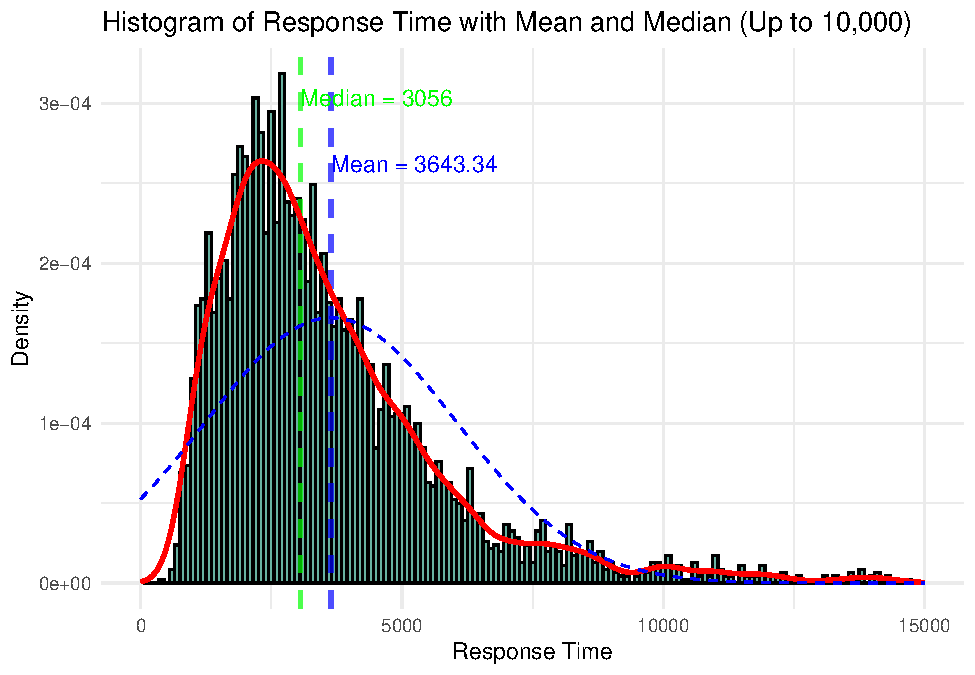
\includegraphics{EDA_DavidMC_files/figure-latex/knitr::opts_chunk$set(warning=FALSE,message=FALSE)-1.pdf}

\begin{Shaded}
\begin{Highlighting}[]
\CommentTok{\# Creating a histogram with mean and median lines, along with density and normal distribution curves}
\FunctionTok{ggplot}\NormalTok{(combined\_data, }\FunctionTok{aes}\NormalTok{(}\AttributeTok{x =}\NormalTok{ freq)) }\SpecialCharTok{+}
  \FunctionTok{geom\_histogram}\NormalTok{(}
    \FunctionTok{aes}\NormalTok{(}\AttributeTok{y =}\NormalTok{ ..density..), }
    \AttributeTok{binwidth =} \DecValTok{100}\NormalTok{, }
    \AttributeTok{fill =} \StringTok{"\#69b3a2"}\NormalTok{, }
    \AttributeTok{color =} \StringTok{"black"}
\NormalTok{  ) }\SpecialCharTok{+}
  \FunctionTok{geom\_vline}\NormalTok{(}
    \FunctionTok{aes}\NormalTok{(}\AttributeTok{xintercept =}\NormalTok{ mean\_freq), }
    \AttributeTok{color =} \StringTok{"blue"}\NormalTok{, }
    \AttributeTok{linetype =} \StringTok{"dashed"}\NormalTok{, }
    \AttributeTok{size =} \DecValTok{1}\NormalTok{, }
    \AttributeTok{alpha =} \FloatTok{0.7}
\NormalTok{  ) }\SpecialCharTok{+}
  \FunctionTok{geom\_vline}\NormalTok{(}
    \FunctionTok{aes}\NormalTok{(}\AttributeTok{xintercept =}\NormalTok{ median\_freq), }
    \AttributeTok{color =} \StringTok{"green"}\NormalTok{, }
    \AttributeTok{linetype =} \StringTok{"dashed"}\NormalTok{, }
    \AttributeTok{size =} \DecValTok{1}\NormalTok{, }
    \AttributeTok{alpha =} \FloatTok{0.7}
\NormalTok{  ) }\SpecialCharTok{+}
  \FunctionTok{xlim}\NormalTok{(}\FunctionTok{c}\NormalTok{(}\DecValTok{0}\NormalTok{, }\DecValTok{200000}\NormalTok{)) }\SpecialCharTok{+}
  \FunctionTok{theme\_minimal}\NormalTok{() }\SpecialCharTok{+}
  \FunctionTok{geom\_density}\NormalTok{(}
    \AttributeTok{color =} \StringTok{"red"}\NormalTok{, }
    \AttributeTok{size =} \DecValTok{1}
\NormalTok{  ) }\SpecialCharTok{+}
  \FunctionTok{stat\_function}\NormalTok{(}
    \AttributeTok{fun =}\NormalTok{ dnorm, }
    \AttributeTok{args =} \FunctionTok{list}\NormalTok{(}
      \AttributeTok{mean =} \FunctionTok{mean}\NormalTok{(combined\_data}\SpecialCharTok{$}\NormalTok{freq, }\AttributeTok{na.rm =} \ConstantTok{TRUE}\NormalTok{), }
      \AttributeTok{sd =} \FunctionTok{sd}\NormalTok{(combined\_data}\SpecialCharTok{$}\NormalTok{freq, }\AttributeTok{na.rm =} \ConstantTok{TRUE}\NormalTok{)}
\NormalTok{    ), }
    \AttributeTok{color =} \StringTok{"blue"}\NormalTok{, }
    \AttributeTok{linetype =} \StringTok{"dashed"}
\NormalTok{  ) }\SpecialCharTok{+}
  \FunctionTok{labs}\NormalTok{(}
    \AttributeTok{title =} \StringTok{"Histogram of Word Frequency with Mean and Median (Up to 10,000)"}\NormalTok{,}
    \AttributeTok{x =} \StringTok{"Word Frequency Rank"}\NormalTok{,}
    \AttributeTok{y =} \StringTok{"Density"}
\NormalTok{  ) }\SpecialCharTok{+}
  \FunctionTok{geom\_text}\NormalTok{(}
    \FunctionTok{aes}\NormalTok{(}\AttributeTok{x =}\NormalTok{ mean\_freq, }\AttributeTok{y =} \DecValTok{0}\NormalTok{, }\AttributeTok{label =} \FunctionTok{paste}\NormalTok{(}\StringTok{"Mean ="}\NormalTok{, }\FunctionTok{round}\NormalTok{(mean\_freq, }\DecValTok{2}\NormalTok{))), }
    \AttributeTok{vjust =} \SpecialCharTok{{-}}\DecValTok{20}\NormalTok{, }
    \AttributeTok{color =} \StringTok{"blue"}\NormalTok{, }
    \AttributeTok{hjust =} \DecValTok{0}\NormalTok{, }
    \AttributeTok{size =} \DecValTok{4}\NormalTok{, }
    \AttributeTok{alpha =} \FloatTok{0.7}
\NormalTok{  ) }\SpecialCharTok{+}
  \FunctionTok{geom\_text}\NormalTok{(}
    \FunctionTok{aes}\NormalTok{(}\AttributeTok{x =}\NormalTok{ median\_freq, }\AttributeTok{y =} \DecValTok{0}\NormalTok{, }\AttributeTok{label =} \FunctionTok{paste}\NormalTok{(}\StringTok{"Median ="}\NormalTok{, }\FunctionTok{round}\NormalTok{(median\_freq, }\DecValTok{2}\NormalTok{))), }
    \AttributeTok{vjust =} \SpecialCharTok{{-}}\DecValTok{20}\NormalTok{, }
    \AttributeTok{color =} \StringTok{"green"}\NormalTok{, }
    \AttributeTok{hjust =} \DecValTok{0}\NormalTok{, }
    \AttributeTok{size =} \DecValTok{4}\NormalTok{, }
    \AttributeTok{alpha =} \FloatTok{0.7}
\NormalTok{  )}
\end{Highlighting}
\end{Shaded}

\begin{verbatim}
## Warning: Removed 1076 rows containing non-finite values (`stat_bin()`).
\end{verbatim}

\begin{verbatim}
## Warning: Removed 1076 rows containing non-finite values (`stat_density()`).
\end{verbatim}

\begin{verbatim}
## Warning: Removed 2 rows containing missing values (`geom_bar()`).
\end{verbatim}

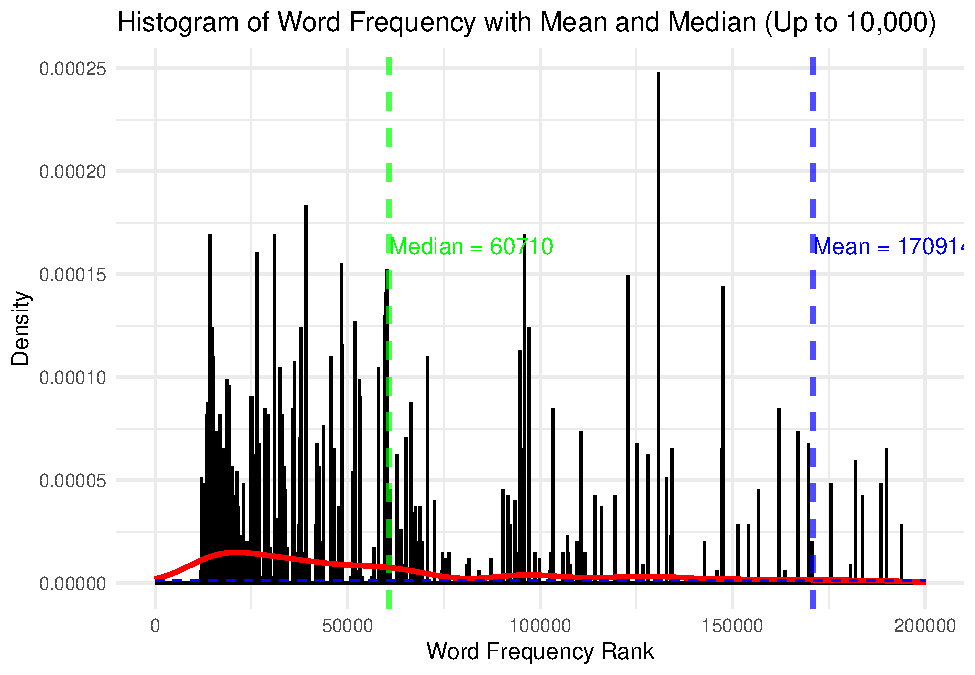
\includegraphics{EDA_DavidMC_files/figure-latex/unnamed-chunk-17-1.pdf}

\hypertarget{q-q-plots-to-check-for-deviations-from-normality}{%
\subsubsection{Q-Q Plots to check for deviations from
normality}\label{q-q-plots-to-check-for-deviations-from-normality}}

\begin{Shaded}
\begin{Highlighting}[]
\FunctionTok{qqnorm}\NormalTok{(combined\_data}\SpecialCharTok{$}\NormalTok{rt, }\AttributeTok{main =} \StringTok{"Q{-}Q Plot for Response Time"}\NormalTok{)}
\FunctionTok{qqline}\NormalTok{(combined\_data}\SpecialCharTok{$}\NormalTok{rt, }\AttributeTok{col =} \StringTok{"red"}\NormalTok{) }\CommentTok{\# Color for visibility}
\end{Highlighting}
\end{Shaded}

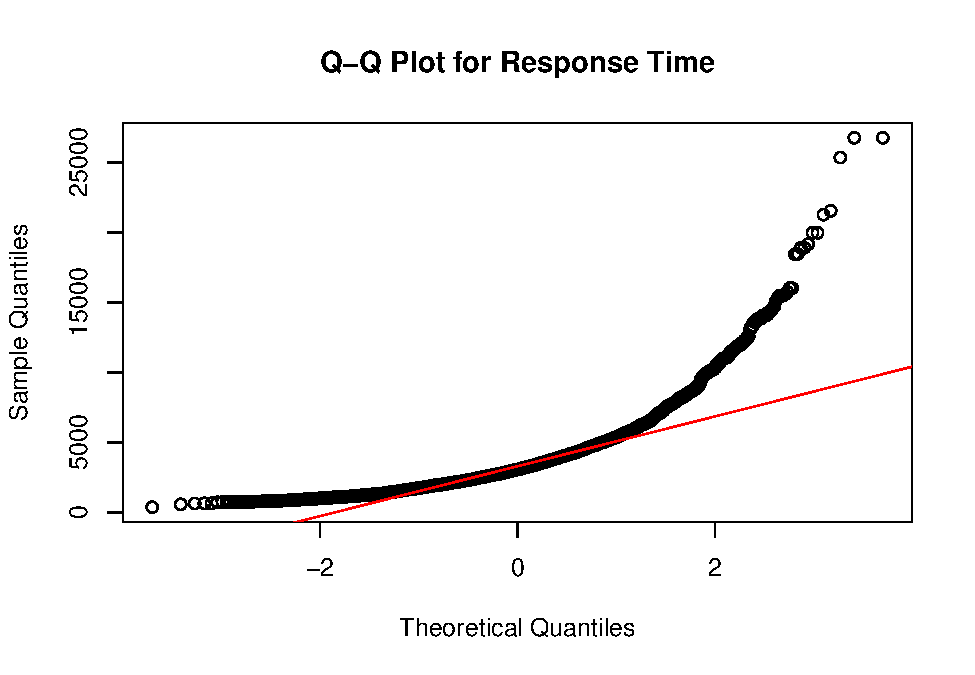
\includegraphics{EDA_DavidMC_files/figure-latex/unnamed-chunk-18-1.pdf}

\begin{Shaded}
\begin{Highlighting}[]
\FunctionTok{qqnorm}\NormalTok{(combined\_data}\SpecialCharTok{$}\NormalTok{freq, }\AttributeTok{main =} \StringTok{"Q{-}Q Plot for Word Fz"}\NormalTok{)}
\FunctionTok{qqline}\NormalTok{(combined\_data}\SpecialCharTok{$}\NormalTok{freq, }\AttributeTok{col =} \StringTok{"red"}\NormalTok{) }\CommentTok{\# Color for visibility}
\end{Highlighting}
\end{Shaded}

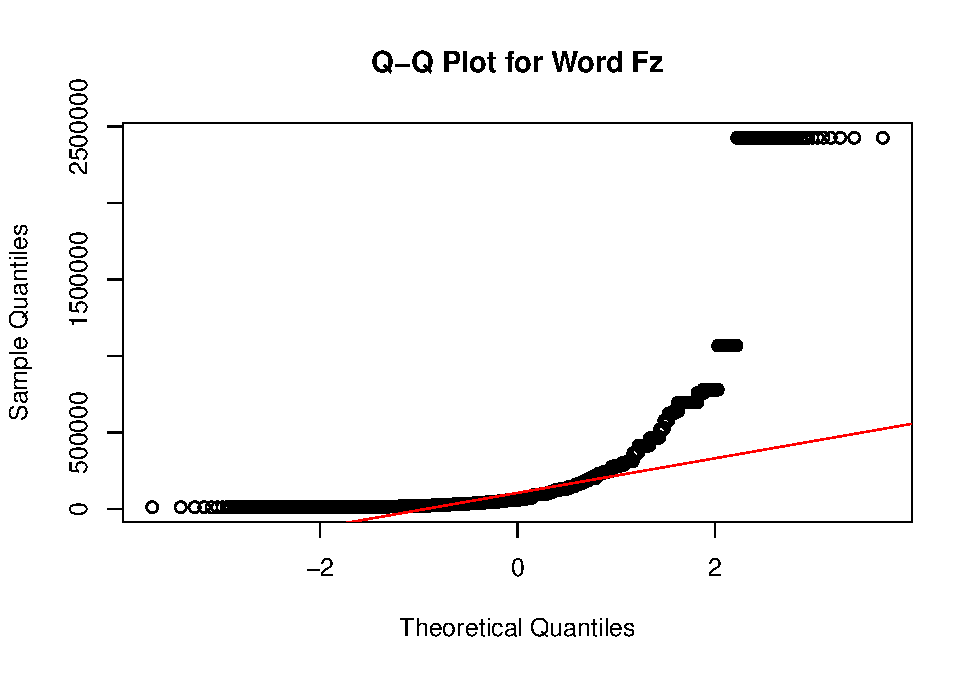
\includegraphics{EDA_DavidMC_files/figure-latex/unnamed-chunk-19-1.pdf}

\hypertarget{visualization-if-there-are-any-correlation-between-word-frequenzy-and-response-time}{%
\subsubsection{Visualization if there are any correlation between Word
Frequenzy and Response
Time}\label{visualization-if-there-are-any-correlation-between-word-frequenzy-and-response-time}}

Before performing the Spearman correlation statistic, we want to
visualize both variables to see if they show signs of correlation
between them.

We have chosen Hexbinplot since with a scatter plot it was very
difficult to visualize in which area there was more density due to the
number of points in the same area. The Hexbin plot suggests that most
responses have a high frequency but we can't observe any correlation
between the frequency of a word and the time response.

\begin{Shaded}
\begin{Highlighting}[]
\FunctionTok{ggplot}\NormalTok{(combined\_data, }\FunctionTok{aes}\NormalTok{(}\AttributeTok{x =}\NormalTok{ freq, }\AttributeTok{y =}\NormalTok{ rt)) }\SpecialCharTok{+}
  \FunctionTok{geom\_hex}\NormalTok{() }\SpecialCharTok{+}
  \FunctionTok{labs}\NormalTok{(}\AttributeTok{title =} \StringTok{"Hexbin Plot of Frequency vs. Response Time"}\NormalTok{,}
       \AttributeTok{x =} \StringTok{"Word Frequency Rank"}\NormalTok{, }\AttributeTok{y =} \StringTok{"Response Time"}\NormalTok{) }\SpecialCharTok{+}
  \FunctionTok{theme\_minimal}\NormalTok{()}
\end{Highlighting}
\end{Shaded}

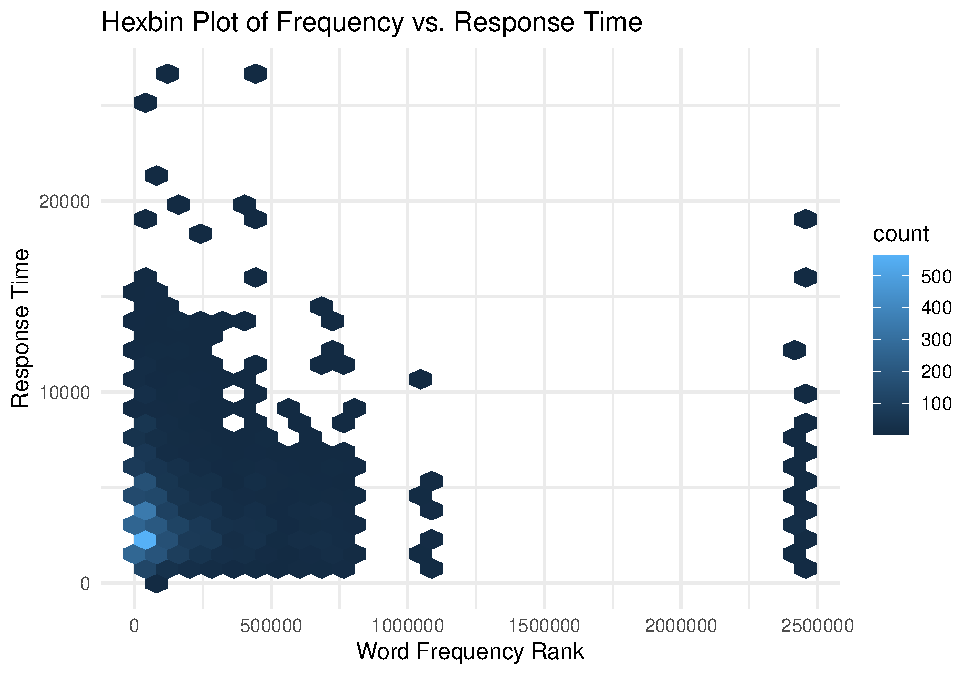
\includegraphics{EDA_DavidMC_files/figure-latex/unnamed-chunk-20-1.pdf}

\hypertarget{correlation-test}{%
\subsubsection{Correlation Test}\label{correlation-test}}

Although there does not seem to be a correlation in the graph, we are
going to use the non-parametric statistic Spearman's rank correlation
coefficient to ensure that there is no significant correlation

\begin{Shaded}
\begin{Highlighting}[]
\NormalTok{cor\_test\_result }\OtherTok{\textless{}{-}} \FunctionTok{cor.test}\NormalTok{(combined\_data}\SpecialCharTok{$}\NormalTok{rt, combined\_data}\SpecialCharTok{$}\NormalTok{freq, }\AttributeTok{method=}\StringTok{"spearman"}\NormalTok{)}
\end{Highlighting}
\end{Shaded}

\begin{verbatim}
## Warning in cor.test.default(combined_data$rt, combined_data$freq, method =
## "spearman"): Cannot compute exact p-value with ties
\end{verbatim}

\begin{Shaded}
\begin{Highlighting}[]
\FunctionTok{print}\NormalTok{(cor\_test\_result)}
\end{Highlighting}
\end{Shaded}

\begin{verbatim}
## 
##  Spearman's rank correlation rho
## 
## data:  combined_data$rt and combined_data$freq
## S = 1.6487e+10, p-value = 0.6553
## alternative hypothesis: true rho is not equal to 0
## sample estimates:
##         rho 
## 0.006558301
\end{verbatim}

\hypertarget{results}{%
\section{RESULTS}\label{results}}

\hypertarget{eda-results}{%
\subsubsection{EDA Results}\label{eda-results}}

We have found a database with many NAs, which reduced the sample
enormously. With data collection that has required meticulous
processing, which can be improved for future research, such as the way
of collecting the responses, where many errors have been found and
instead of classifying the two experiments in a column and in another
put the answers, we have found: \{``let\_linear'':``able''\}, which had
to be separated into two columns and cleaned. Worrying response times
have also been found that reduce the internal and external validity of
the experiment, with a Mean Response Time: 3643.337 and a Standard
Deviation of Response Time: 2403.828.

The Corpus of Contemporary American English (COCA) is a very interesting
data set because it not only has the frequency of words in general, but
also classifies them by categories, giving rise to interesting future
research.

\hypertarget{correlation-results}{%
\subsubsection{Correlation Results}\label{correlation-results}}

The Spearman's rank correlation test result shows a rho value of
approximately 0.0066, suggesting a very weak positive correlation
between response time and word frequency. However, the p-value of 0.6553
suggests that this correlation is not statistically significant, meaning
there's no strong evidence of a monotonic relationship between the two
variables in the sample data.

\hypertarget{visualizing-the-spearmans-rank-correlation-coefficient}{%
\subsubsection{Visualizing the Spearman's rank correlation
coefficient}\label{visualizing-the-spearmans-rank-correlation-coefficient}}

\begin{Shaded}
\begin{Highlighting}[]
\CommentTok{\# \# We first need to calculate the ranks of the data}
\NormalTok{combined\_data}\SpecialCharTok{$}\NormalTok{rank\_rt }\OtherTok{\textless{}{-}} \FunctionTok{rank}\NormalTok{(combined\_data}\SpecialCharTok{$}\NormalTok{rt, }\AttributeTok{ties.method =} \StringTok{"average"}\NormalTok{)}
\NormalTok{combined\_data}\SpecialCharTok{$}\NormalTok{rank\_freq }\OtherTok{\textless{}{-}} \FunctionTok{rank}\NormalTok{(combined\_data}\SpecialCharTok{$}\NormalTok{freq, }\AttributeTok{ties.method =} \StringTok{"average"}\NormalTok{)}

\CommentTok{\# Now create a scatter plot of these ranks}
\FunctionTok{ggplot}\NormalTok{(combined\_data, }\FunctionTok{aes}\NormalTok{(}\AttributeTok{x =}\NormalTok{ rank\_rt, }\AttributeTok{y =}\NormalTok{ rank\_freq)) }\SpecialCharTok{+}
  \FunctionTok{geom\_point}\NormalTok{() }\SpecialCharTok{+}
  \FunctionTok{geom\_smooth}\NormalTok{(}\AttributeTok{method =} \StringTok{"lm"}\NormalTok{, }\AttributeTok{se =} \ConstantTok{FALSE}\NormalTok{) }\SpecialCharTok{+}
  \FunctionTok{labs}\NormalTok{(}\AttributeTok{x =} \StringTok{"Rank of Response Time"}\NormalTok{, }\AttributeTok{y =} \StringTok{"Rank of Word Frequency"}\NormalTok{, }
       \AttributeTok{title =} \StringTok{"Scatter plot of Ranks with Spearman\textquotesingle{}s Correlation"}\NormalTok{) }\SpecialCharTok{+}
  \FunctionTok{theme\_minimal}\NormalTok{()}
\end{Highlighting}
\end{Shaded}

\begin{verbatim}
## `geom_smooth()` using formula = 'y ~ x'
\end{verbatim}

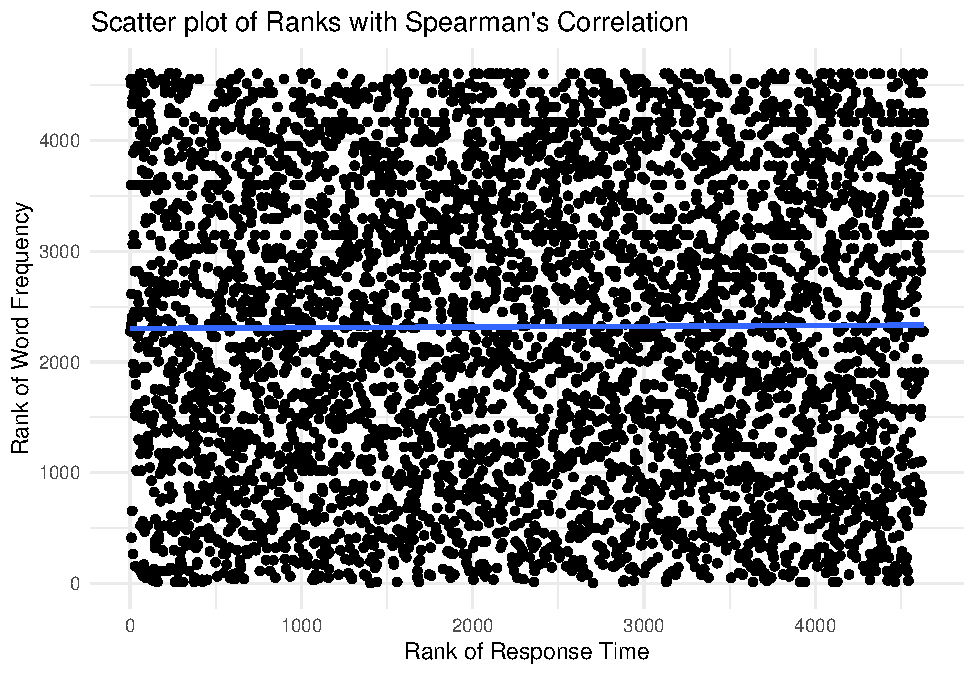
\includegraphics{EDA_DavidMC_files/figure-latex/unnamed-chunk-22-1.pdf}

The scatter plot shows the ranks of response time on the x-axis and the
ranks of word frequency on the y-axis. Each point represents a pair of
ranks, and the plot is a visual representation of the Spearman's rank
correlation.

The blue line across the plot appears to be a best-fit line through the
data points, which should be flat because the ranks of response time and
word frequency are plotted against each other. The flatness of the line
suggests there is very little to no monotonic relationship between the
two ranks, which aligns with the previously mentioned Spearman
correlation coefficient of approximately 0.0066 and the high p-value.

The dense clustering of points along the entire range of ranks without a
clear upward or downward trend further supports the conclusion of a very
weak correlation. This means that knowing the rank of a word's frequency
does not provide much information about the rank of the response time in
this dataset.

\hypertarget{discussion}{%
\section{DISCUSSION}\label{discussion}}

We have found that there appears to be no correlation between response
time and word frequency. But also exploring the database, we have seen
certain limitations that may be interfering in the validity of our
analyses, such as that since it is an online experiment there is no type
of supervision by any researcher, response times are very high. In
general, there was no time limit set, and there are many variables that
can interfere with this reaction time such as internet problems, typing
speed, distractors around while taking the test, and multiple variables
that have not already been controlled. which was not the original goal
of the experiments. Therefore, it is important to interpret the results
taking these limitations into account. From here it is invited to carry
out more controlled tests in future research and to carry out the
analysis of the semantic distance between words, to see if relationships
are found between the semantic distances and the response time, which
would be more in line with the foraging effect that is studied in the
original paper of this data set.

The results of this analysis are of utmost importance because they will
help us design better experiments where we can control many more
variables, generate better databases and study the phenomenon of
semantic memory recovery with more detail and scientific rigor.

\hypertarget{references}{%
\section{REFERENCES}\label{references}}

Graf, P., \& Mandler, G. (1984). Activation makes words more accessible,
but not necessarily more retrievable. Journal of Verbal Learning and
Verbal Behavior, 23(5), 553--568.
\url{https://doi.org/10.1016/S0022-5371(84)90346-3}

Hills, T. T., Jones, M. N., \& Todd, P. M. (2012). Optimal foraging in
semantic memory. Psychological Review, 119(2), 431.
\url{http://dx.doi.org/10.1037/a0027373}

Malaie, S., Spivey, M., \& Marghetis, T. (2023). Divergent and
Convergent Creativity Are Different Kinds of Foraging.

Peng, D., \& Elizabeth, M. (2015). ``The Art of Data Science.'' A Guide
for Anyone Who Works with Data. Skybrude Consulting, LLC.

Sánchez, A., Carreiras, M., \& Paz-Alonso, P. M. (2023). Word frequency
and reading demands modulate brain activation in the inferior frontal
gyrus. Scientific Reports, 13(1), 17217.

Warrington, E. K., \& Weiskrantz, L. (1970). Amnesic syndrome:
Consolidation or retrieval? Nature, 228(5272), 628--630.
\url{https://doi.org/10.1038/228628a0}

\end{document}
